\section{Numerical examples}
\label{section: Chapter4/examples}

In this section, we study in detail the formation of crack networks in thin films and soil desiccation.  We begin
in \Cref{section: Chapter4/examples/1D} with a deterministic benchmark problem under quasi-one-dimensional conditions.  The spacing between fractures is calculated as a function of the driving force with the cohesive fracture model and compared against a linear elasticity solution.
Attention is then turned to an investigation of the stochastic aspects of fracture with a two-dimensional plane stress model in \Cref{section: Chapter4/examples/2D}, wherein the fracture toughness and critical fracture energy are modeled as random fields.
Finally, in \Cref{section: Chapter4/examples/3D} we present stochastic simulations of a soil desiccation process in three dimensions.

%%%%%%%%%%%%%%%%%%%%%%%%%%%%%%%%%%%%%%%%%%%%%%%%%%%%%%%%%%%%%%%%%%%%%%%%%%%%%%%%%%%%%%%%%%%
%%%%%%%%%%%%%%%%%%%%%%%%%%%%%%%%%%%%%%%%%%%%%%%%%%%%%%%%%%%%%%%%%%%%%%%%%%%%%%%%%%%%%%%%%%%
%%%%%%%%%%%%%%%%%%%%%%%%%%%%%%%%%%%%%%%%%%%%%%%%%%%%%%%%%%%%%%%%%%%%%%%%%%%%%%%%%%%%%%%%%%%
%%%%%%%%%%%%%%%%%%%%%%%%%%%%%%%%%%%%%%%%%%%%%%%%%%%%%%%%%%%%%%%%%%%%%%%%%%%%%%%%%%%%%%%%%%%
%%%%%%%%%%%%%%%%%%%%%%%%%%%%%%%%%%%%%%%%%%%%%%%%%%%%%%%%%%%%%%%%%%%%%%%%%%%%%%%%%%%%%%%%%%%
%%%%%%%%%%%%%%%%%%%%%%%%%%%%%%%%%%%%%%%%%%%%%%%%%%%%%%%%%%%%%%%%%%%%%%%%%%%%%%%%%%%%%%%%%%%
%%%%%%%%%%%%%%%%%%%%%%%%%%%%%%%%%%%%%%%%%%%%%%%%%%%%%%%%%%%%%%%%%%%%%%%%%%%%%%%%%%%%%%%%%%%
%%%%%%%%%%%%%%%%%%%%%%%%%%%%%%%%%%%%%%%%%%%%%%%%%%%%%%%%%%%%%%%%%%%%%%%%%%%%%%%%%%%%%%%%%%%
%%%%%%%%%%%%%%%%%%%%%%%%%%%%%%%%%%%%%%%%%%%%%%%%%%%%%%%%%%%%%%%%%%%%%%%%%%%%%%%%%%%%%%%%%%%
%%%%%%%%%%%%%%%%%%%%%%%%%%%%%%%%%%%%%%%%%%%%%%%%%%%%%%%%%%%%%%%%%%%%%%%%%%%%%%%%%%%%%%%%%%%
\subsection{One-Dimensional Simplification: Side View}
\label{section: Chapter4/examples/1D}

We begin by deriving an analytical solution for the fracture of a thin film bonded to a thick substrate, as shown in \Cref{fig: Chapter4/1D/simplification}.  Assuming that the planar dimensions of the film are much larger than its thickness, we first simplify the problem into a two-dimensional (or quasi 1D) plane-strain problem. The film is assumed to have Young's modulus $E_1$, Poisson's ratio $\nu_1$, and thickness $h$. The substrate has Young's modulus $E_0$, Poisson's ratio $\nu_0$, and thickness $H$.  The fracture of the film is driven by the underlying substrate being stretched an amount $\varepsilon_x$.  The problem with these simplifications and assumptions has been studied by many researchers, and analytical solutions from elasticity theory have been derived in several different ways.  The derivation presented herein most closely follows that provided in \citet{yin2008explicit}.

\begin{figure}
  \centering
  \begin{subfigure}[b]{0.35\textwidth}
    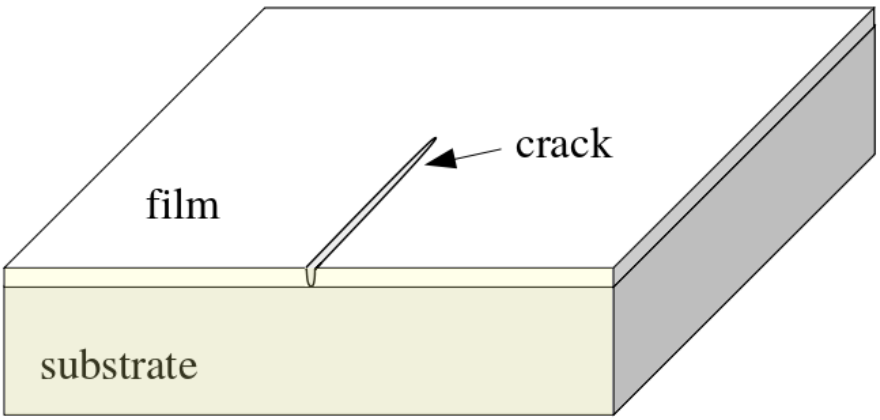
\includegraphics[width=\textwidth,scale=0.5]{Chapter4/figures/1D/side_view.png}
    \caption{}
  \end{subfigure}
  \begin{subfigure}[b]{0.45\textwidth}
    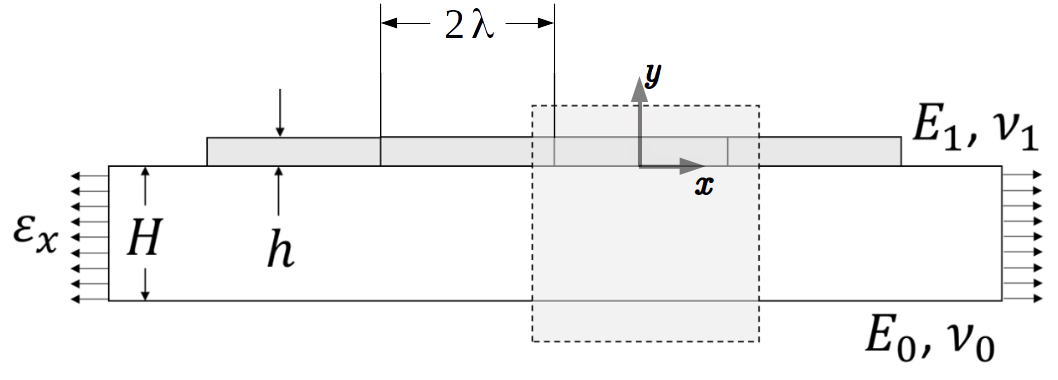
\includegraphics[width=\textwidth,scale=0.5]{Chapter4/figures/1D/1D_schematic.png}
    \caption{}
    \label{fig: Chapter4/1D/schematic}
  \end{subfigure}
  \caption{Description of a one-dimensional model for thin-film cracking.  (a) Side view  (highlighted in yellow) of the geometry (b) schematic representation of the side view. The elasticity solution is derived for the region highlighted with the shaded box, i.e.\ between the two discontinuities across the thin film. The coordinate system is centered at the middle of the bottom surface of the thin film. }
  \label{fig: Chapter4/1D/simplification}
\end{figure}


\begin{figure}
  \centering
  \begin{overpic}[scale=0.55]{Chapter4/figures/1D/supersuperposition.png}
    \put(12,-4){(a)}
    \put(46,-4){(b)}
    \put(80,-4){(c)}
  \end{overpic}
  \vspace{0.2in}
  \caption{ The principal of ``super-superposition'' applied to the region of interest marked in \Cref{fig: Chapter4/1D/schematic}. The analytical solution is derived based on the boundary conditions shown in (c). }
  \label{fig: Chapter4/1D/supersuperposition}
\end{figure}


With the increase of the tensile strain in the substrate, some uniformly distributed discontinuities with spacing $2\lambda$ form across the thickness of the film. We assume that no debonding occurs and that the vertical component of the displacement does not vary in the horizontal direction, i.e.
\begin{align}
  u_y(x,y) = u_y(y) .
\end{align}
The plane-strain equilibrium equation in the x--direction is written as
\begin{align}
  \dfrac{E_1}{1-\nu_1^2}u_{x,xx} + \mu_1u_{x,yy} = 0 ,
\end{align}
where $\mu_1$ denotes the shear modulus of the film.  This is supplemented by appropriate boundary conditions (\Cref{fig: Chapter4/1D/supersuperposition})
\begin{align}
  u_x(0,y)                                                    & = 0 ,                                    \\
  u_{x,y}(x,h)                                                & = 0 ,                                    \\
  \dfrac{1}{h}\int\limits_{0}^h \sigma_x(\lambda,y)\text{ d}y & = -\dfrac{E_1}{1-\nu_1^2}\varepsilon_x . 
\end{align}
We obtain the closed-form solution to the displacement field
\begin{align}
  u_x(x,y) = \varepsilon_xx-\dfrac{\sinh(cx/h)}{\cosh(c\lambda/h)}\dfrac{\cos(d(1-y/h))}{\sin(d)}\sqrt{\dfrac{E_1}{\mu_1(1-\nu_1^2)}}h\varepsilon_x ,
\end{align}
where $c$ and $d$ are functions of Dundur's parameters $\alpha$ and $\beta$. Following \cite{BEUTH19921657,xia2000crack,yin2008explicit}, $c$ and $d$ can be computed as:
\begin{align}
   & c = \dfrac{2}{\pi k(\alpha,\beta)}, \quad d = \sqrt{\dfrac{2}{1-\nu_1}}c ,                                                                          \\
   & \alpha = \dfrac{\Bar{E}_1-\Bar{E}_0}{\Bar{E}_1+\Bar{E}_0}, \quad \beta = \dfrac{\mu_1(1-2\nu_0)-\mu_0(1-2\nu_1)}{2\mu_1(1-\nu_0)+2\mu_0(1-\nu_1)} , \\
   & k(\alpha,\beta) \approx k(\alpha) = \dfrac{1.258-0.4\alpha-0.26\alpha^3-0.3\alpha^4}{1-\alpha} ,                                                    
\end{align}
with $\Bar{E}_0 = \dfrac{E_0}{(1-\nu_0^2)}$, and $\Bar{E}_1 = \dfrac{E_1}{(1-\nu_1^2)}$. By replacing $\lambda$ with $\lambda/2$, the crack opening displacement can be written as
\begin{align}
  \delta(0,y) = 2\tanh\left(\dfrac{c\lambda}{2h}\right)\dfrac{\cos(d(1-y/h))}{\sin(d)}\sqrt{\dfrac{E_1}{\mu_1(1-\nu_1^2)}}h\varepsilon_x .
\end{align}
Then the fracture toughness can be obtained as the work done to close the crack, i.e.
\begin{align}
  \mathcal{G}_c\cdot2h & = \int\limits_0^h \sigma_x(0,y)\delta(0,y)\text{ d}y,                                                                                                          \\
  \mathcal{G}_c        & = \dfrac{(1-\nu_1^2)\sigma_x^2}{E_1}\dfrac{h}{c}\left[ 2\tanh\left( \dfrac{c\lambda}{2h} \right)-\tanh(c\lambda/h) \right] .\label{eq: 1D analytical solution} 
\end{align}
The amount of energy released by opening a transverse crack is governed by two dimensionless parameters:
\begin{align}
  \mathcal{D}^* = \sqrt{\dfrac{(1-\nu_1^2)h}{E_1\mathcal{G}_c}}\sigma_x, \quad l^* = \dfrac{\lambda}{h} \label{eq: dimensionless parameters}.
\end{align}
It is then convenient to interpret the  parameter $\mathcal{D}^*$ as the dimensionless fracture driving energy and $l^*$ as the dimensionless crack spacing. \eqref{eq: 1D analytical solution} can be rendered dimensionless following \eqref{eq: dimensionless parameters}, and the relation between the dimensionless fracture driving energy and the dimensionless crack spacing can be written as
\begin{align}
  \mathcal{D}^* \mathcal{C}(l^*;c) = 1, \quad \mathcal{C}(l^*;c) = \dfrac{1}{c}\left[ 2\tanh\left( \dfrac{1}{2} c l^* \right)-\tanh(cl^*) \right].
\end{align}

\begin{figure}[htbp!]
  \centering
  \begin{subfigure}[b]{0.45\textwidth}
    \centering
    \tikzsetnextfilenamesafe{Chapter4/1D/analytical}
    \begin{tikzpicture}
      \begin{axis}[
          cycle list name=exotic,
          width=\textwidth,
          height=1\textwidth,
          xmode=log,
          log ticks with fixed point,
          xlabel=$l^*$,ylabel=$\mathcal{D}^*$,
          ymin=0,ymax=2.5,
          legend style={at={(0.95,0.95)},anchor=north east},
          legend style={nodes={scale=0.6, transform shape}},
          legend cell align={left},
          every axis plot/.append style={thick}
        ]
        \addplot +[mark=none] table {Chapter4/data/1D/0.5_analytical.csv};
        \addplot +[mark=none] table {Chapter4/data/1D/1_analytical.csv};
        \addplot +[mark=none] table {Chapter4/data/1D/2_analytical.csv};
        \addplot +[mark=none] table {Chapter4/data/1D/5_analytical.csv};
        \addplot +[mark=none] table {Chapter4/data/1D/10_analytical.csv};
        \legend{$E_0/E_1 = 0.5$,$E_0/E_1 = 1$,$E_0/E_1 = 2$,$E_0/E_1 = 5$,$E_0/E_1 = 10$}
      \end{axis}
    \end{tikzpicture}
    \caption{}
    \label{fig: Chapter4/1D/analytical}
  \end{subfigure}
  \begin{subfigure}[b]{0.45\textwidth}
    \centering
    \tikzsetnextfilenamesafe{Chapter4/1D/numerical}
    \begin{tikzpicture}
      \begin{axis}[
          cycle list name=exotic,
          width=\textwidth,
          height=1\textwidth,
          xmode=log,
          log ticks with fixed point,
          xlabel=$l^*$,ylabel=$\mathcal{D}^*$,
          ymin=0,ymax=2.5,
          legend style={at={(0.95,0.95)},anchor=north east},
          legend style={nodes={scale=0.6, transform shape}},
          legend cell align={left},
          every axis plot/.append style={thick,mark size=1pt}
        ]
        \addplot table {Chapter4/data/1D/0.5_numerical.csv};
        \addplot table {Chapter4/data/1D/1_numerical.csv};
        \addplot table {Chapter4/data/1D/2_numerical.csv};
        \addplot table {Chapter4/data/1D/5_numerical.csv};
        \addplot table {Chapter4/data/1D/10_numerical.csv};
        \legend{$E_0/E_1 = 0.5$,$E_0/E_1 = 1$,$E_0/E_1 = 2$,$E_0/E_1 = 5$,$E_0/E_1 = 10$}
      \end{axis}
    \end{tikzpicture}
    \caption{}
    \label{fig: Chapter4/1D/numerical}
  \end{subfigure}
  \caption[Relationship  between the dimensionless fracture driving energy and the dimensionless crack spacing.]{Relationship  between the dimensionless fracture driving energy and the dimensionless crack spacing: (a) analytical solution using linear elasticity; and (b) numerically generated curves using the phase-field for cohesive model detailed in this work. }
  \label{fig: Chapter4/1D/compare_analytical_numerical}
\end{figure}


In \Cref{fig: Chapter4/1D/analytical}, we set the Poisson's ratio of both the film and the substrate to be $\nu_0 = \nu_1 = 0.2$, and plot the dimensionless fracture driving energy versus the dimensionless crack spacing for different combinations of the mismatch in the Young's modulus between the film and the substrate.

Next, we performed a series of numerical simulations using the phase-field model for cohesive fracture following the setup described in \Cref{fig: Chapter4/1D/schematic}.  Specifically, we examine the amount of driving energy required to propagate one transverse crack through the thickness of the film. The substrate and the film are represented by two rectangular domains $\body_s = [-\lambda,\lambda] \times [\SI{-5}{\milli\meter},0]$
and $\body_f = [-\lambda,\lambda] \times [0,\SI{1}{\milli\meter}]$, repsectively. The film-substrate system is the union of the two, i.e.\ $\body_0 = \body_s \cup \body_f$, and left-right periodicity is enforced. The substrate and the film are discretized with linear triangular elements with characteristic lengths of $h^e_s = \lambda/10$ and $h^e_f = \lambda/100$, respectively.
The numerical results (\Cref{fig: Chapter4/1D/numerical}) show a good agreement with the analytical solution.

%%%%%%%%%%%%%%%%%%%%%%%%%%%%%%%%%%%%%%%%%%%%%%%%%%%%%%%%%%%%%%%%%%%%%%%%%%%%%%%%%%%%%%%%%%%
%%%%%%%%%%%%%%%%%%%%%%%%%%%%%%%%%%%%%%%%%%%%%%%%%%%%%%%%%%%%%%%%%%%%%%%%%%%%%%%%%%%%%%%%%%%
%%%%%%%%%%%%%%%%%%%%%%%%%%%%%%%%%%%%%%%%%%%%%%%%%%%%%%%%%%%%%%%%%%%%%%%%%%%%%%%%%%%%%%%%%%%
%%%%%%%%%%%%%%%%%%%%%%%%%%%%%%%%%%%%%%%%%%%%%%%%%%%%%%%%%%%%%%%%%%%%%%%%%%%%%%%%%%%%%%%%%%%
%%%%%%%%%%%%%%%%%%%%%%%%%%%%%%%%%%%%%%%%%%%%%%%%%%%%%%%%%%%%%%%%%%%%%%%%%%%%%%%%%%%%%%%%%%%
%%%%%%%%%%%%%%%%%%%%%%%%%%%%%%%%%%%%%%%%%%%%%%%%%%%%%%%%%%%%%%%%%%%%%%%%%%%%%%%%%%%%%%%%%%%
%%%%%%%%%%%%%%%%%%%%%%%%%%%%%%%%%%%%%%%%%%%%%%%%%%%%%%%%%%%%%%%%%%%%%%%%%%%%%%%%%%%%%%%%%%%
%%%%%%%%%%%%%%%%%%%%%%%%%%%%%%%%%%%%%%%%%%%%%%%%%%%%%%%%%%%%%%%%%%%%%%%%%%%%%%%%%%%%%%%%%%%
%%%%%%%%%%%%%%%%%%%%%%%%%%%%%%%%%%%%%%%%%%%%%%%%%%%%%%%%%%%%%%%%%%%%%%%%%%%%%%%%%%%%%%%%%%%
%%%%%%%%%%%%%%%%%%%%%%%%%%%%%%%%%%%%%%%%%%%%%%%%%%%%%%%%%%%%%%%%%%%%%%%%%%%%%%%%%%%%%%%%%%%
\subsection{Two-Dimensional Simplification: Stochastic Aspects of Fracture}
\label{section: Chapter4/examples/2D}

We now consider a two-dimensional model of a thin film on a substrate wherein the geometry of the resulting fracture patterns is considerably more complex.  For the bulk material properties, we adopt values that are representative of clay. The material properties and model parameters are summarized in \Cref{tab: clay}.

We focus attention on the sensitivity of the resulting fracture patterns to stochastic spatial variations in the fracture properties. The random field of fracture properties $\{(\Gc(\btX),\psi_c(\btX)), \btX \in \body_0\}$ is defined and sampled following the model and procedures presented in \Cref{section: Chapter4/theory/stochastic}. For all cases, the spatial correlation length $L$ is larger than the regularization length $l$ of the phase-field model. A tolerance of $1 \times 10^{-3}$ is chosen for the truncation error in the Karhunen-Lo\`{e}ve expansion \eqref{eq: truncation}.
The mean values of $\Gc$ and $\psi_c$ are chosen in accordance with reported values for clay as listed in \Cref{tab: clay}. Coefficients of variation are chosen to be $0.03$, leading to a variation of about $\pm 10\%$ around the mean value for the two random fracture parameters. All realizations shown in figures are normalized with respect to the corresponding stationary mean function, and the normalized quantities are denoted by $\Gc^*$ and $\psi_c^*$.

\begin{table}[htb!]
  \centering
  \caption{Summary of material properties and model parameters for all calculations in \Cref{section: Chapter4/examples/2D}}
  \begin{tabular}{r c c c c}
    \toprule
    Property/Parameter            & Symbol                      & Value & Unit                                & Comment                                       \\
    \midrule
    Young's modulus               & $E$                         & 4     & \SI{}{\mega\pascal}                 & See \cite{obrzud2010hardening, Rodriguez2006} \\
    Poisson's ratio               & $\nu$                       & 0.2   & nondim.                             & See \cite{obrzud2010hardening, Rodriguez2006} \\
    Mean fracture toughness       & $\underline{\mathcal{G}_c}$ & 27    & \SI{}{\kilo\joule\per\square\meter} & See \cite{ramsaroop2010fracture}              \\[5pt]
    Mean critical fracture energy & $\underline{\psi_c}$        & 30    & \SI{}{\joule\per\square\meter}      & See \cite{ramsaroop2010fracture}              \\[5pt]
    Regularization length         & $l$                         & 0.5   & \SI{}{\milli\meter}                 & Such that $2l/h^e \approx 5$                  \\
    Degradation shape parameter   & $p$                         & 1     & nondim.                             &                                               \\
    \bottomrule
  \end{tabular}
  \label{tab: clay}
\end{table}

%%%%%%%%%%%%%%%%%%%%%%%%%%%%%%%%%%%%%%%%%%%%%%%%%%%%%%%%%%%%%%%%%%%%%%%%%%%%%%%%%%%%%%%%%%%
%%%%%%%%%%%%%%%%%%%%%%%%%%%%%%%%%%%%%%%%%%%%%%%%%%%%%%%%%%%%%%%%%%%%%%%%%%%%%%%%%%%%%%%%%%%
%%%%%%%%%%%%%%%%%%%%%%%%%%%%%%%%%%%%%%%%%%%%%%%%%%%%%%%%%%%%%%%%%%%%%%%%%%%%%%%%%%%%%%%%%%%
%%%%%%%%%%%%%%%%%%%%%%%%%%%%%%%%%%%%%%%%%%%%%%%%%%%%%%%%%%%%%%%%%%%%%%%%%%%%%%%%%%%%%%%%%%%
%%%%%%%%%%%%%%%%%%%%%%%%%%%%%%%%%%%%%%%%%%%%%%%%%%%%%%%%%%%%%%%%%%%%%%%%%%%%%%%%%%%%%%%%%%%
%%%%%%%%%%%%%%%%%%%%%%%%%%%%%%%%%%%%%%%%%%%%%%%%%%%%%%%%%%%%%%%%%%%%%%%%%%%%%%%%%%%%%%%%%%%
%%%%%%%%%%%%%%%%%%%%%%%%%%%%%%%%%%%%%%%%%%%%%%%%%%%%%%%%%%%%%%%%%%%%%%%%%%%%%%%%%%%%%%%%%%%
%%%%%%%%%%%%%%%%%%%%%%%%%%%%%%%%%%%%%%%%%%%%%%%%%%%%%%%%%%%%%%%%%%%%%%%%%%%%%%%%%%%%%%%%%%%
%%%%%%%%%%%%%%%%%%%%%%%%%%%%%%%%%%%%%%%%%%%%%%%%%%%%%%%%%%%%%%%%%%%%%%%%%%%%%%%%%%%%%%%%%%%
%%%%%%%%%%%%%%%%%%%%%%%%%%%%%%%%%%%%%%%%%%%%%%%%%%%%%%%%%%%%%%%%%%%%%%%%%%%%%%%%%%%%%%%%%%%
\subsubsection{A Plane-Stress Model}

We now consider the problem of a thin film of thickness $h$ that is bonded to an elastic underlayer of thickness $H$, as shown in Figure \ref{fig: Chapter4/2D/simplification}.  The entire structure is assumed to be bonded to a rigid substrate. For this case, we employ the shear-lag model that is detailed in \cite{liang2003evolving}.  The square domain is discretized using linear triangular elements with a characteristic length of $h^e = a/500$. This  mesh is used for the displacement subproblem, the phase-field subproblem for fracture, and the generalized eigenvalue problem for the random fields. The displacement field and the phase field are constrained to be $a-$periodic, and the random fields are constructed to be $a-$periodic as well.

\begin{figure}[htb!]
  \centering
  \begin{subfigure}[b]{0.35\textwidth}
    \centering
    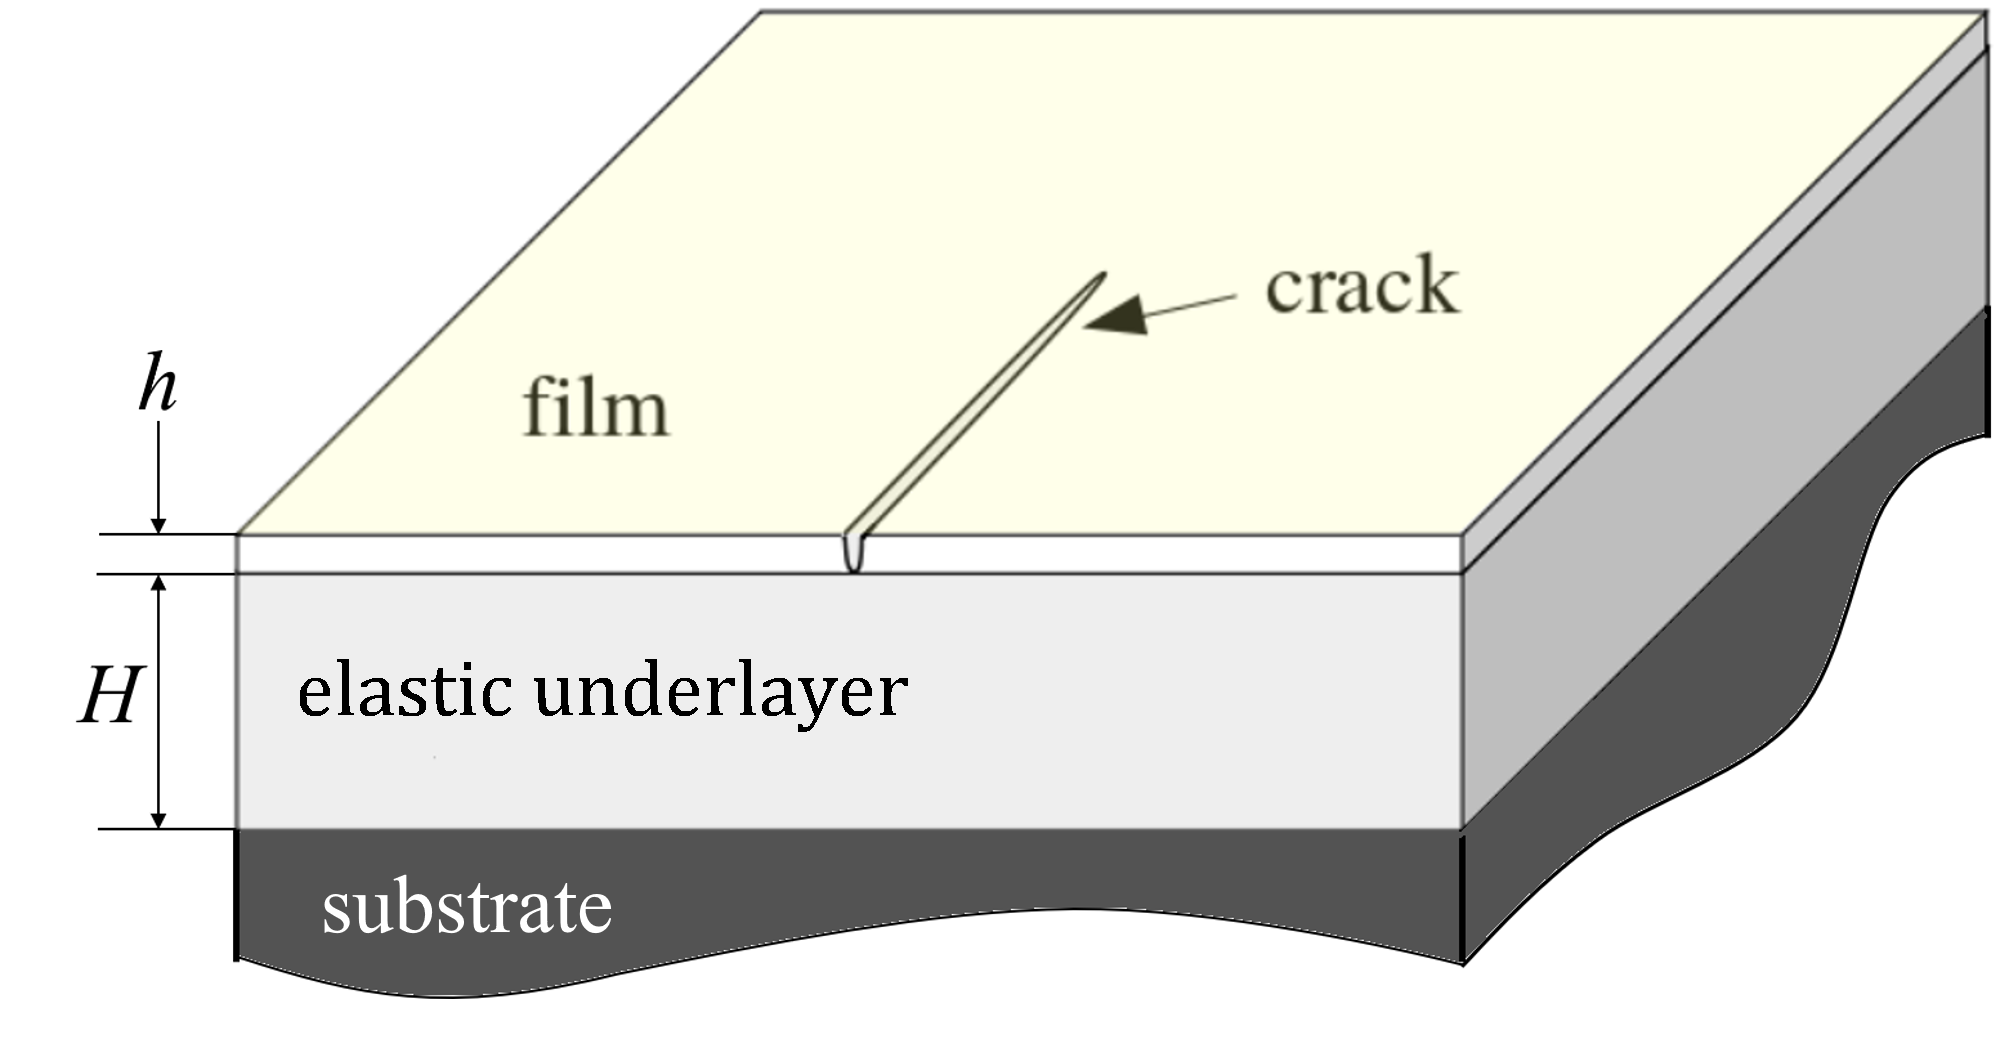
\includegraphics[width=\textwidth,scale=0.5]{Chapter4/figures/2D/top_view.png}
    \caption{}
  \end{subfigure}
  \hspace{0.1\textwidth}
  \begin{subfigure}[b]{0.3\textwidth}
    \centering
    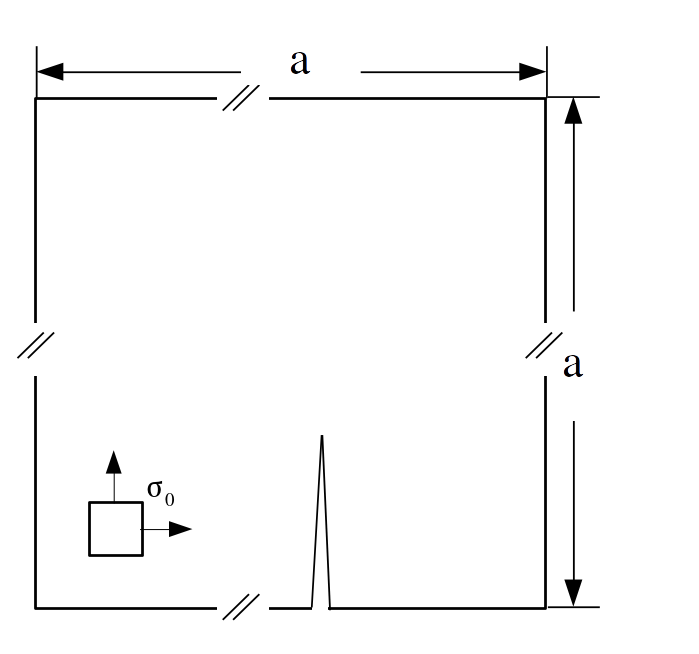
\includegraphics[width=\textwidth,scale=0.5]{Chapter4/figures/2D/2D_schematic.png}
    \caption{}
  \end{subfigure}
  \caption[Description of a two-dimensional model for thin-film cracking.]{Description of a two-dimensional model for thin-film cracking. (a) Top view (highlighted in yellow) (b) schematic representation of the top view. A typical crack is shown to emphasize that fracture is only considered in the film. }
  \label{fig: Chapter4/2D/simplification}
\end{figure}


%%%%%%%%%%%%%%%%%%%%%%%%%%%%%%%%%%%%%%%%%%%%%%%%%%%%%%%%%%%%%%%%%%%%%%%%%%%%%%%%%%%%%%%%%%%
%%%%%%%%%%%%%%%%%%%%%%%%%%%%%%%%%%%%%%%%%%%%%%%%%%%%%%%%%%%%%%%%%%%%%%%%%%%%%%%%%%%%%%%%%%%
%%%%%%%%%%%%%%%%%%%%%%%%%%%%%%%%%%%%%%%%%%%%%%%%%%%%%%%%%%%%%%%%%%%%%%%%%%%%%%%%%%%%%%%%%%%
%%%%%%%%%%%%%%%%%%%%%%%%%%%%%%%%%%%%%%%%%%%%%%%%%%%%%%%%%%%%%%%%%%%%%%%%%%%%%%%%%%%%%%%%%%%
%%%%%%%%%%%%%%%%%%%%%%%%%%%%%%%%%%%%%%%%%%%%%%%%%%%%%%%%%%%%%%%%%%%%%%%%%%%%%%%%%%%%%%%%%%%
%%%%%%%%%%%%%%%%%%%%%%%%%%%%%%%%%%%%%%%%%%%%%%%%%%%%%%%%%%%%%%%%%%%%%%%%%%%%%%%%%%%%%%%%%%%
%%%%%%%%%%%%%%%%%%%%%%%%%%%%%%%%%%%%%%%%%%%%%%%%%%%%%%%%%%%%%%%%%%%%%%%%%%%%%%%%%%%%%%%%%%%
%%%%%%%%%%%%%%%%%%%%%%%%%%%%%%%%%%%%%%%%%%%%%%%%%%%%%%%%%%%%%%%%%%%%%%%%%%%%%%%%%%%%%%%%%%%
%%%%%%%%%%%%%%%%%%%%%%%%%%%%%%%%%%%%%%%%%%%%%%%%%%%%%%%%%%%%%%%%%%%%%%%%%%%%%%%%%%%%%%%%%%%
%%%%%%%%%%%%%%%%%%%%%%%%%%%%%%%%%%%%%%%%%%%%%%%%%%%%%%%%%%%%%%%%%%%%%%%%%%%%%%%%%%%%%%%%%%%
\subsubsection{Effect of Correlation Length and Smoothness}

To study the effect of the correlation length, crack patterns for four different values of $L$ are compared. Ten calculations, corresponding to ten samples of the stochastic fields, are carried out for each value of $L$. Representative random fields and their corresponding phase fields are shown in \Cref{fig: Chapter4/2D/compare_correlation_length}.

\begin{figure}[!htbp]
  \centering
  \begin{subfigure}[b]{0.45\textwidth}
    \caption*{Squared Exponential Kernel}
  \end{subfigure}
  \begin{subfigure}[b]{0.45\textwidth}
    \caption*{Exponential Kernel}
  \end{subfigure}
  
  \begin{subfigure}[b]{0.15\textwidth}
    \caption*{$\Gc^*$}
    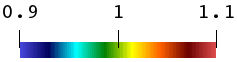
\includegraphics[width=\textwidth]{Chapter4/figures/rainbow_horizontal.png}
  \end{subfigure}
  \begin{subfigure}[b]{0.15\textwidth}
    \caption*{$\psi_c^*$}
    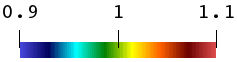
\includegraphics[width=\textwidth]{Chapter4/figures/rainbow_horizontal.png}
  \end{subfigure}
  \begin{subfigure}[b]{0.15\textwidth}
    \caption*{$d$}
    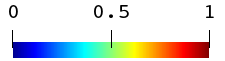
\includegraphics[width=\textwidth]{Chapter4/figures/jet_horizontal.png}
  \end{subfigure}
  \begin{subfigure}[b]{0.15\textwidth}
    \caption*{$\Gc^*$}
    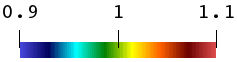
\includegraphics[width=\textwidth]{Chapter4/figures/rainbow_horizontal.png}
  \end{subfigure}
  \begin{subfigure}[b]{0.15\textwidth}
    \caption*{$\psi_c^*$}
    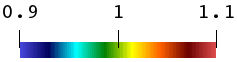
\includegraphics[width=\textwidth]{Chapter4/figures/rainbow_horizontal.png}
  \end{subfigure}
  \begin{subfigure}[b]{0.15\textwidth}
    \caption*{$d$}
    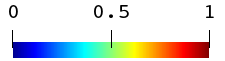
\includegraphics[width=\textwidth]{Chapter4/figures/jet_horizontal.png}
  \end{subfigure}
  
  \begin{subfigure}[b]{0.15\textwidth}
    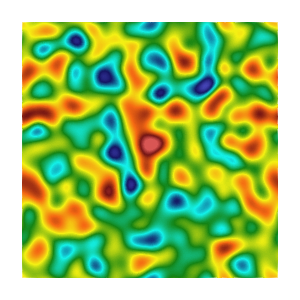
\includegraphics[width=\textwidth]{Chapter4/figures/2D/Gc_sqexp_cartesian_5_5_rho_0_seed_a.png}
    \caption{$L^* = 0.05$}
    \label{fig: Chapter4/2D/Gc_sqexp_cartesian_5_5_rho_0_seed_a}
  \end{subfigure}
  \begin{subfigure}[b]{0.15\textwidth}
    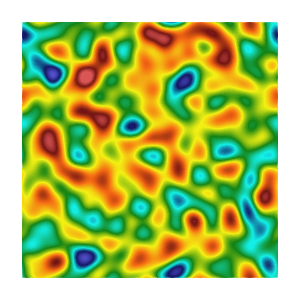
\includegraphics[width=\textwidth]{Chapter4/figures/2D/psic_sqexp_cartesian_5_5_rho_0_seed_a.png}
    \caption{$L^* = 0.05$}
    \label{fig: Chapter4/2D/psic_sqexp_cartesian_5_5_rho_0_seed_a}
  \end{subfigure}
  \begin{subfigure}[b]{0.15\textwidth}
    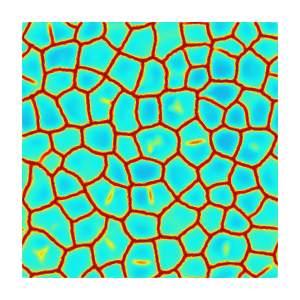
\includegraphics[width=\textwidth]{Chapter4/figures/2D/d_sqexp_cartesian_5_5_rho_0_seed_a.png}
    \caption{}
    \label{fig: Chapter4/2D/d_sqexp_cartesian_5_5_rho_0_seed_a}
  \end{subfigure}
  \begin{subfigure}[b]{0.15\textwidth}
    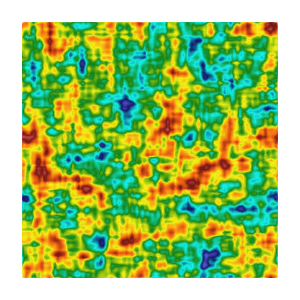
\includegraphics[width=\textwidth]{Chapter4/figures/2D/Gc_exp_cartesian_5_5_rho_0_seed_b.png}
    \caption{$L^* = 0.05$}
    \label{fig: Chapter4/2D/Gc_exp_cartesian_5_5_rho_0_seed_b}
  \end{subfigure}
  \begin{subfigure}[b]{0.15\textwidth}
    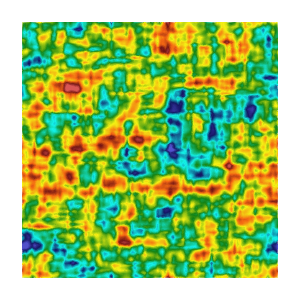
\includegraphics[width=\textwidth]{Chapter4/figures/2D/psic_exp_cartesian_5_5_rho_0_seed_b.png}
    \caption{$L^* = 0.05$}
    \label{fig: Chapter4/2D/psic_exp_cartesian_5_5_rho_0_seed_b}
  \end{subfigure}
  \begin{subfigure}[b]{0.15\textwidth}
    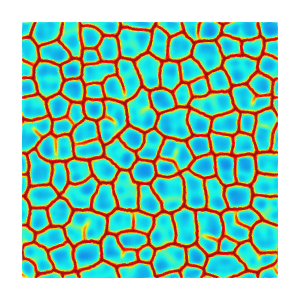
\includegraphics[width=\textwidth]{Chapter4/figures/2D/d_exp_cartesian_5_5_rho_0_seed_b.png}
    \caption{}
    \label{fig: Chapter4/2D/d_exp_cartesian_5_5_rho_0_seed_b}
  \end{subfigure}
  
  \begin{subfigure}[b]{0.15\textwidth}
    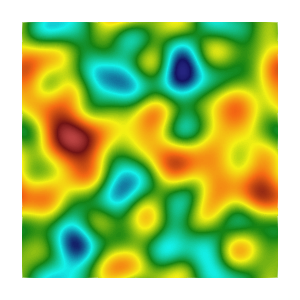
\includegraphics[width=\textwidth]{Chapter4/figures/2D/Gc_sqexp_cartesian_10_10_rho_0_seed_a.png}
    \caption{$L^* = 0.1$}
    \label{fig: Chapter4/2D/Gc_sqexp_cartesian_10_10_rho_0_seed_a}
  \end{subfigure}
  \begin{subfigure}[b]{0.15\textwidth}
    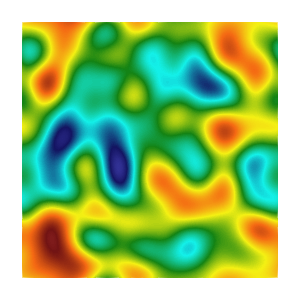
\includegraphics[width=\textwidth]{Chapter4/figures/2D/psic_sqexp_cartesian_10_10_rho_0_seed_a.png}
    \caption{$L^* = 0.1$}
    \label{fig: Chapter4/2D/psic_sqexp_cartesian_10_10_rho_0_seed_a}
  \end{subfigure}
  \begin{subfigure}[b]{0.15\textwidth}
    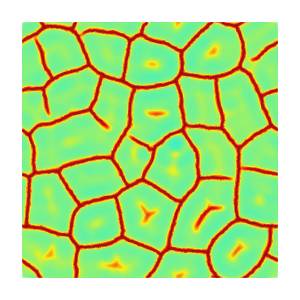
\includegraphics[width=\textwidth]{Chapter4/figures/2D/d_sqexp_cartesian_10_10_rho_0_seed_a.png}
    \caption{}
    \label{fig: Chapter4/2D/d_sqexp_cartesian_10_10_rho_0_seed_a}
  \end{subfigure}
  \begin{subfigure}[b]{0.15\textwidth}
    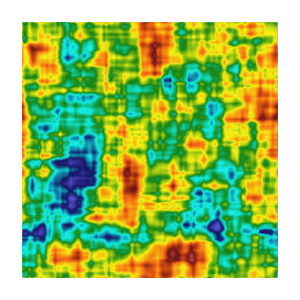
\includegraphics[width=\textwidth]{Chapter4/figures/2D/Gc_exp_cartesian_10_10_rho_0_seed_b.png}
    \caption{$L^* = 0.1$}
    \label{fig: Chapter4/2D/Gc_exp_cartesian_10_10_rho_0_seed_b}
  \end{subfigure}
  \begin{subfigure}[b]{0.15\textwidth}
    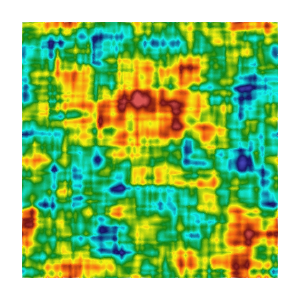
\includegraphics[width=\textwidth]{Chapter4/figures/2D/psic_exp_cartesian_10_10_rho_0_seed_b.png}
    \caption{$L^* = 0.1$}
    \label{fig: Chapter4/2D/psic_exp_cartesian_10_10_rho_0_seed_b}
  \end{subfigure}
  \begin{subfigure}[b]{0.15\textwidth}
    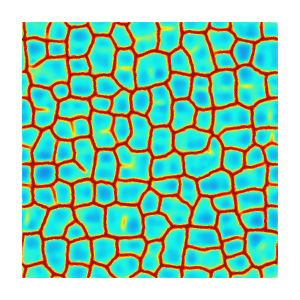
\includegraphics[width=\textwidth]{Chapter4/figures/2D/d_exp_cartesian_10_10_rho_0_seed_b.png}
    \caption{}
    \label{fig: Chapter4/2D/d_exp_cartesian_10_10_rho_0_seed_b}
  \end{subfigure}
  
  \begin{subfigure}[b]{0.15\textwidth}
    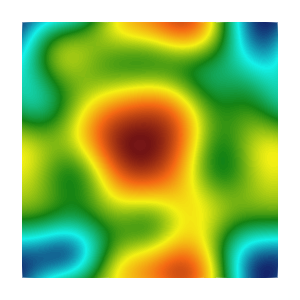
\includegraphics[width=\textwidth]{Chapter4/figures/2D/Gc_sqexp_cartesian_20_20_rho_0_seed_a.png}
    \caption{$L^* = 0.2$}
    \label{fig: Chapter4/2D/Gc_sqexp_cartesian_20_20_rho_0_seed_a}
  \end{subfigure}
  \begin{subfigure}[b]{0.15\textwidth}
    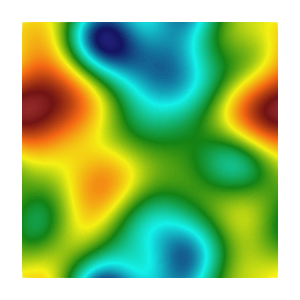
\includegraphics[width=\textwidth]{Chapter4/figures/2D/psic_sqexp_cartesian_20_20_rho_0_seed_a.png}
    \caption{$L^* = 0.2$}
    \label{fig: Chapter4/2D/psic_sqexp_cartesian_20_20_rho_0_seed_a}
  \end{subfigure}
  \begin{subfigure}[b]{0.15\textwidth}
    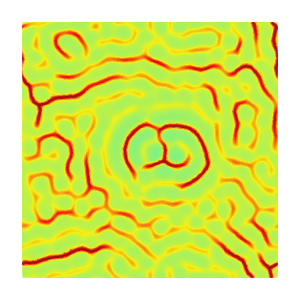
\includegraphics[width=\textwidth]{Chapter4/figures/2D/d_sqexp_cartesian_20_20_rho_0_seed_a.png}
    \caption{}
    \label{fig: Chapter4/2D/d_sqexp_cartesian_20_20_rho_0_seed_a}
  \end{subfigure}
  \begin{subfigure}[b]{0.15\textwidth}
    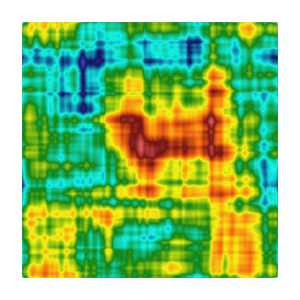
\includegraphics[width=\textwidth]{Chapter4/figures/2D/Gc_exp_cartesian_20_20_rho_0_seed_b.png}
    \caption{$L^* = 0.2$}
    \label{fig: Chapter4/2D/Gc_exp_cartesian_20_20_rho_0_seed_b}
  \end{subfigure}
  \begin{subfigure}[b]{0.15\textwidth}
    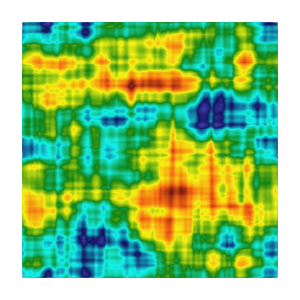
\includegraphics[width=\textwidth]{Chapter4/figures/2D/psic_exp_cartesian_20_20_rho_0_seed_b.png}
    \caption{$L^* = 0.2$}
    \label{fig: Chapter4/2D/psic_exp_cartesian_20_20_rho_0_seed_b}
  \end{subfigure}
  \begin{subfigure}[b]{0.15\textwidth}
    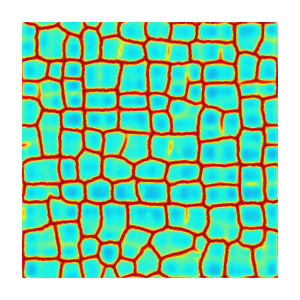
\includegraphics[width=\textwidth]{Chapter4/figures/2D/d_exp_cartesian_20_20_rho_0_seed_b.png}
    \caption{}
    \label{fig: Chapter4/2D/d_exp_cartesian_20_20_rho_0_seed_b}
  \end{subfigure}
  \caption[Phase fields resulting from six pairs of realizations with different correlation models and normalized correlation lengths.]{Phase fields resulting from six pairs of realizations with different correlation models and normalized correlation lengths. The left three pairs (a-b, g-h, m-n) are realizations obtained with a PSE covariance function, while the right three pairs (d-e, j-k, p-q) are samples generated with a PE covariance function. Energy release rate $\Gc$ and the critical fracture energy $\psi_c$ have a coefficient of variation of $0.03$, and normalized spatial correlation length $L^*$ of (a-b, d-e) $0.05$ (g-h, j-k) $0.1$ (m-n, p-q) $0.2$ The corresponding phase fields are shown in (c, f, i, l, o, r), respectively. In these results, independent realizations of the underlying Gaussian fields are used.}
  \label{fig: Chapter4/2D/compare_correlation_length}
\end{figure}


\begin{figure}[htbp!]
  \centering
  \begin{subfigure}[b]{0.475\textwidth}
    \centering
    \tikzsetnextfilenamesafe{Chapter4/2D/dimensionless_curve_correlation_length_sqexp}
    \begin{tikzpicture}
      \begin{axis}[
          width=0.9\textwidth,
          height=1.1\textwidth,
          ymode=log,
          log ticks with fixed point,
          ylabel=$\underline{l^*}$,xlabel=$\mathcal{D}^*$,
          % ymin=0,ymax=2.5,
          legend style={
              at={(0.05,0.05)},
              anchor=south west,
              nodes={scale=1, transform shape},
              fill=none,
              draw=none,
              text opacity=1,
              cells={align=left}
            },
          legend cell align={left},
          every axis plot/.append style={thick}
        ]
        % sqexp l = 5
        \addplot [select coords between index={40}{220},color=black] table [x expr=\thisrowno{0},y expr=\thisrowno{1}]{Chapter4/data/2D/dimensionless_curve_sqexp_cartesian_5_5.csv};
        % sqexp l = 10
        \addplot [select coords between index={40}{220},color=red] table [x expr=\thisrowno{0},y expr=\thisrowno{1}]{Chapter4/data/2D/dimensionless_curve_sqexp_cartesian_10_10.csv};
        % sqexp l = 20
        \addplot [select coords between index={40}{220},color=blue] table [x expr=\thisrowno{0},y expr=\thisrowno{1}]{Chapter4/data/2D/dimensionless_curve_sqexp_cartesian_20_20.csv};
        \legend{sqexp $L^* = 0.05$,sqexp $L^* = 0.1$,sqexp $L^* = 0.2$}
      \end{axis}
    \end{tikzpicture}
    \caption{}
    \label{fig: Chapter4/2D/dimensionless_curve_correlation_length_sqexp}
  \end{subfigure}
  \begin{subfigure}[b]{0.475\textwidth}
    \centering
    \tikzsetnextfilenamesafe{Chapter4/2D/distribution_correlation_length_sqexp}
    \begin{tikzpicture}
      \begin{axis}[
          width=0.9\textwidth,
          height=1.1\textwidth,
          xlabel=$l^*$,ylabel=estimated PDF,
          ymin=0,ymax=0.012,
          xmin=0,xmax=1000,
          legend style={at={(0.95,0.95)},anchor=north east},
          legend style={nodes={scale=1, transform shape}},
          legend style={fill=none,draw=none},
          legend cell align={left},
          every axis plot/.append style={thick}
        ]
        \addplot [color=black] table [x expr=\thisrowno{0},y expr=\thisrowno{1}]{Chapter4/data/2D/distribution_sqexp_cartesian_5_5.csv};
        \addplot [color=red] table [x expr=\thisrowno{0},y expr=\thisrowno{1}]{Chapter4/data/2D/distribution_sqexp_cartesian_10_10.csv};
        \addplot [color=blue] table [x expr=\thisrowno{0},y expr=\thisrowno{1}]{Chapter4/data/2D/distribution_sqexp_cartesian_20_20.csv};
        \legend{sqexp $L^* = 0.05$,sqexp $L^* = 0.1$,sqexp $L^* = 0.2$}
      \end{axis}
    \end{tikzpicture}
    \caption{}
    \label{fig: Chapter4/2D/distribution_correlation_length_sqexp}
  \end{subfigure}
  
  \begin{subfigure}[b]{0.475\textwidth}
    \centering
    \tikzsetnextfilenamesafe{Chapter4/2D/dimensionless_curve_correlation_length_exp}
    \begin{tikzpicture}
      \begin{axis}[
          width=0.9\textwidth,
          height=1.1\textwidth,
          ymode=log,
          log ticks with fixed point,
          ylabel=$\underline{l^*}$,xlabel=$\mathcal{D}^*$,
          % ymin=0,ymax=2.5,
          legend style={
              at={(0.05,0.05)},
              anchor=south west,
              nodes={scale=1, transform shape},
              fill=none,
              draw=none,
              text opacity=1,
              cells={align=left}
            },
          legend cell align={left},
          every axis plot/.append style={thick}
        ]
        % sqexp l = 5
        \addplot [select coords between index={40}{220},color=black] table [x expr=\thisrowno{0},y expr=\thisrowno{1}]{Chapter4/data/2D/dimensionless_curve_exp_cartesian_5_5.csv};
        % sqexp l = 10
        \addplot [select coords between index={40}{220},color=red] table [x expr=\thisrowno{0},y expr=\thisrowno{1}]{Chapter4/data/2D/dimensionless_curve_exp_cartesian_10_10.csv};
        % sqexp l = 20
        \addplot [select coords between index={40}{220},color=blue] table [x expr=\thisrowno{0},y expr=\thisrowno{1}]{Chapter4/data/2D/dimensionless_curve_exp_cartesian_20_20.csv};
        \legend{exp $L^* = 0.05$,exp $L^* = 0.1$,exp $L^* = 0.2$}
      \end{axis}
    \end{tikzpicture}
    \caption{}
    \label{fig: Chapter4/2D/dimensionless_curve_correlation_length_exp}
  \end{subfigure}
  \begin{subfigure}[b]{0.475\textwidth}
    \centering
    \tikzsetnextfilenamesafe{Chapter4/2D/distribution_correlation_length_exp}
    \begin{tikzpicture}
      \begin{axis}[
          width=0.9\textwidth,
          height=1.1\textwidth,
          xlabel=$l^*$,ylabel=estimated PDF,
          ymin=0,ymax=0.012,
          xmin=0,xmax=300,
          legend style={at={(0.95,0.95)},anchor=north east},
          legend style={nodes={scale=1, transform shape}},
          legend style={fill=none,draw=none},
          legend cell align={left},
          every axis plot/.append style={thick}
        ]
        \addplot [color=black] table [x expr=\thisrowno{0},y expr=\thisrowno{1}]{Chapter4/data/2D/distribution_exp_cartesian_5_5.csv};
        \addplot [color=red] table [x expr=\thisrowno{0},y expr=\thisrowno{1}]{Chapter4/data/2D/distribution_exp_cartesian_10_10.csv};
        \addplot [color=blue] table [x expr=\thisrowno{0},y expr=\thisrowno{1}]{Chapter4/data/2D/distribution_exp_cartesian_20_20.csv};
        \legend{exp $L^* = 0.05$,exp $L^* = 0.1$,exp $L^* = 0.2$}
      \end{axis}
    \end{tikzpicture}
    \caption{}
    \label{fig: Chapter4/2D/distribution_correlation_length_exp}
  \end{subfigure}
  \caption[Fragment statistics for different values of correlation length.]{(a, c) Mean dimensionless crack spacing $\underline{l^*}$ versus dimensionless crack driving force $\mathcal{D}^*$ (b, d) Estimated probability density of dimensionless crack spacing for different values of correlation length when $\mathcal{D}^* = 5.17$ based on (a-b) a PSE kernel (c-d) a PE kernel }
  \label{fig: Chapter4/2D/statistics_correlation_length}
\end{figure}


A Flooding algorithm (described in \Cref{appendix: flooding}) is used to group elements into clusters in a volume-preserving way, to facilitate the counting of distinct fragments. Following the one-dimensional derivation (\Cref{section: Chapter4/examples/1D}), two dimensionless parameters are extracted as
\begin{align}
   & \mathcal{D}^* = \sqrt{\dfrac{(1-\nu_1^2)h}{E_1\underline{\mathcal{G}_c}}}\sigma_0, \quad l^* = \dfrac{\lambda}{h}, \quad \lambda \approx \sqrt{A} , 
\end{align}
where the crack spacing $\lambda$ is estimated from the fragment area $A$. Dimensionless curves are plotted in \Cref{fig: Chapter4/2D/statistics_correlation_length}.

As expected, it is seen that the PSE covariance model generates smoother realizations. As the normalized correlation length $L^* = L/p$ becomes larger, i.e.\ \Cref{fig: Chapter4/2D/d_sqexp_cartesian_5_5_rho_0_seed_a,fig: Chapter4/2D/d_sqexp_cartesian_10_10_rho_0_seed_a,fig: Chapter4/2D/d_sqexp_cartesian_20_20_rho_0_seed_a},
a substantial amount of damage accumulates before localization occurs to form a ``crack''. When the sample exhibits less spatial fluctuations, a non-negligible portion of the energy is dissipated into the matrix in the form of diffuse damage, resulting in fewer cracks and larger fragment sizes. As the normalized correlation gets even larger, i.e.\ \Cref{fig: Chapter4/2D/Gc_sqexp_cartesian_20_20_rho_0_seed_a,fig: Chapter4/2D/psic_sqexp_cartesian_20_20_rho_0_seed_a,fig: Chapter4/2D/d_sqexp_cartesian_20_20_rho_0_seed_a}, morphologically different crack networks are obtained.

On the other hand, the rougher samples generated using the PE covariance function, i.e.\ \Cref{fig: Chapter4/2D/Gc_exp_cartesian_5_5_rho_0_seed_b,fig: Chapter4/2D/psic_exp_cartesian_5_5_rho_0_seed_b,fig: Chapter4/2D/d_exp_cartesian_5_5_rho_0_seed_b,fig: Chapter4/2D/Gc_exp_cartesian_10_10_rho_0_seed_b,fig: Chapter4/2D/psic_exp_cartesian_10_10_rho_0_seed_b,fig: Chapter4/2D/d_exp_cartesian_10_10_rho_0_seed_b,fig: Chapter4/2D/Gc_exp_cartesian_20_20_rho_0_seed_b,fig: Chapter4/2D/psic_exp_cartesian_20_20_rho_0_seed_b,fig: Chapter4/2D/d_exp_cartesian_20_20_rho_0_seed_b}, have sufficient variations that serve as effective imperfections for damage localization. In terms of the mean size of fragments that form, the corresponding phase fields are seen to be far less sensitive to the spatial correlation length.  However, as the correlation length increases, the orientation of the phase fields begins to acquire a structure that aligns with the axes of the domain. This observation is in accordance with the tensor-product structure of the covariance model, and with the fact that larger correlation lengths allow more pronounced spatial structures to develop (sample-wise) for PE functions.

\begin{figure}[!htb]
  \centering
  \begin{subfigure}[b]{0.45\textwidth}
    \caption*{Squared Exponential Kernel}
  \end{subfigure}
  \begin{subfigure}[b]{0.45\textwidth}
    \caption*{Exponential Kernel}
  \end{subfigure}

  \begin{subfigure}[b]{0.15\textwidth}
    \caption*{$\Gc^*$}
    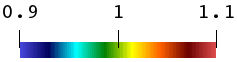
\includegraphics[width=\textwidth]{Chapter4/figures/rainbow_horizontal.png}
  \end{subfigure}
  \begin{subfigure}[b]{0.15\textwidth}
    \caption*{$\psi_c^*$}
    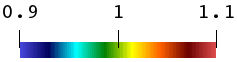
\includegraphics[width=\textwidth]{Chapter4/figures/rainbow_horizontal.png}
  \end{subfigure}
  \begin{subfigure}[b]{0.15\textwidth}
    \caption*{$d$}
    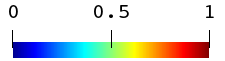
\includegraphics[width=\textwidth]{Chapter4/figures/jet_horizontal.png}
  \end{subfigure}
  \begin{subfigure}[b]{0.15\textwidth}
    \caption*{$\Gc^*$}
    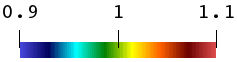
\includegraphics[width=\textwidth]{Chapter4/figures/rainbow_horizontal.png}
  \end{subfigure}
  \begin{subfigure}[b]{0.15\textwidth}
    \caption*{$\psi_c^*$}
    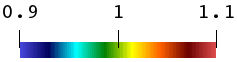
\includegraphics[width=\textwidth]{Chapter4/figures/rainbow_horizontal.png}
  \end{subfigure}
  \begin{subfigure}[b]{0.15\textwidth}
    \caption*{$d$}
    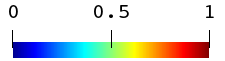
\includegraphics[width=\textwidth]{Chapter4/figures/jet_horizontal.png}
  \end{subfigure}

  \begin{subfigure}[b]{0.15\textwidth}
    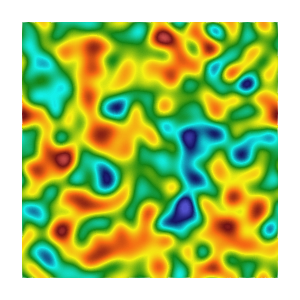
\includegraphics[width=\textwidth]{Chapter4/figures/2D/Gc_sqexp_cartesian_5_5_rho_0_seed_c.png}
    \caption{}
    \label{fig: Chapter4/2D/Gc_sqexp_cartesian_5_5_rho_0_seed_c}
  \end{subfigure}
  \begin{subfigure}[b]{0.15\textwidth}
    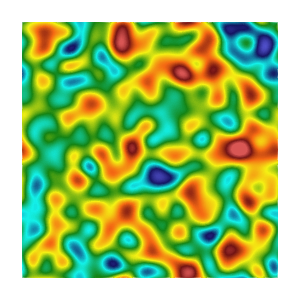
\includegraphics[width=\textwidth]{Chapter4/figures/2D/psic_sqexp_cartesian_5_5_rho_0_seed_c.png}
    \caption{}
    \label{fig: Chapter4/2D/psic_sqexp_cartesian_5_5_rho_0_seed_c}
  \end{subfigure}
  \begin{subfigure}[b]{0.15\textwidth}
    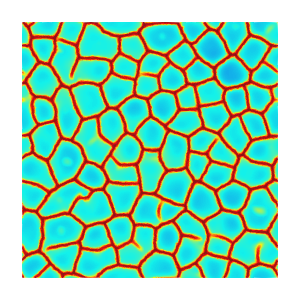
\includegraphics[width=\textwidth]{Chapter4/figures/2D/d_sqexp_cartesian_5_5_rho_0_seed_c.png}
    \caption{}
    \label{fig: Chapter4/2D/d_sqexp_cartesian_5_5_rho_0_seed_c}
  \end{subfigure}
  \begin{subfigure}[b]{0.15\textwidth}
    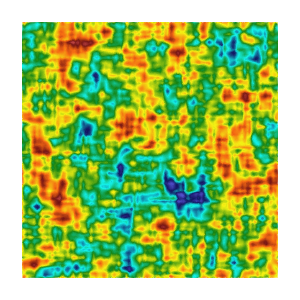
\includegraphics[width=\textwidth]{Chapter4/figures/2D/Gc_exp_cartesian_5_5_rho_0_seed_c.png}
    \caption{}
    \label{fig: Chapter4/2D/Gc_exp_cartesian_5_5_rho_0_seed_c}
  \end{subfigure}
  \begin{subfigure}[b]{0.15\textwidth}
    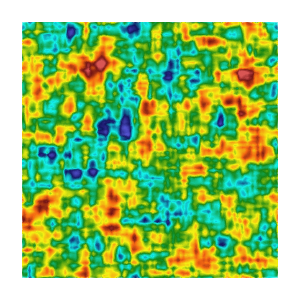
\includegraphics[width=\textwidth]{Chapter4/figures/2D/psic_exp_cartesian_5_5_rho_0_seed_c.png}
    \caption{}
    \label{fig: Chapter4/2D/psic_exp_cartesian_5_5_rho_0_seed_c}
  \end{subfigure}
  \begin{subfigure}[b]{0.15\textwidth}
    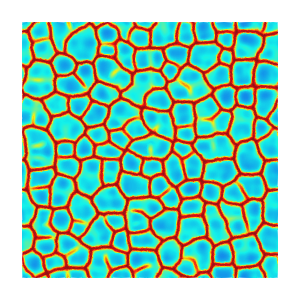
\includegraphics[width=\textwidth]{Chapter4/figures/2D/d_exp_cartesian_5_5_rho_0_seed_c.png}
    \caption{}
    \label{fig: Chapter4/2D/d_exp_cartesian_5_5_rho_0_seed_c}
  \end{subfigure}

  \begin{subfigure}[b]{0.15\textwidth}
    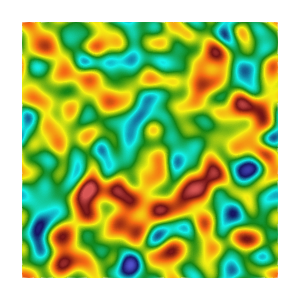
\includegraphics[width=\textwidth]{Chapter4/figures/2D/Gc_sqexp_cartesian_5_5_rho_0_seed_d.png}
    \caption{}
    \label{fig: Chapter4/2D/Gc_sqexp_cartesian_5_5_rho_0_seed_d}
  \end{subfigure}
  \begin{subfigure}[b]{0.15\textwidth}
    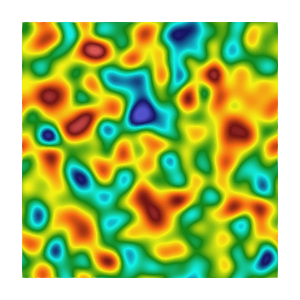
\includegraphics[width=\textwidth]{Chapter4/figures/2D/psic_sqexp_cartesian_5_5_rho_0_seed_d.png}
    \caption{}
    \label{fig: Chapter4/2D/psic_sqexp_cartesian_5_5_rho_0_seed_d}
  \end{subfigure}
  \begin{subfigure}[b]{0.15\textwidth}
    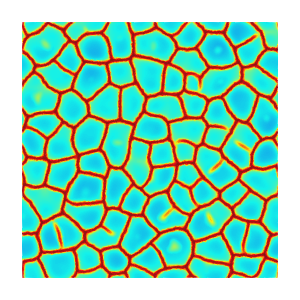
\includegraphics[width=\textwidth]{Chapter4/figures/2D/d_sqexp_cartesian_5_5_rho_0_seed_d.png}
    \caption{}
    \label{fig: Chapter4/2D/d_sqexp_cartesian_5_5_rho_0_seed_d}
  \end{subfigure}
  \begin{subfigure}[b]{0.15\textwidth}
    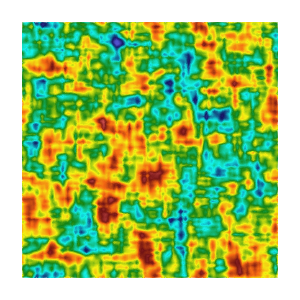
\includegraphics[width=\textwidth]{Chapter4/figures/2D/Gc_exp_cartesian_5_5_rho_0_seed_d.png}
    \caption{}
    \label{fig: Chapter4/2D/Gc_exp_cartesian_5_5_rho_0_seed_d}
  \end{subfigure}
  \begin{subfigure}[b]{0.15\textwidth}
    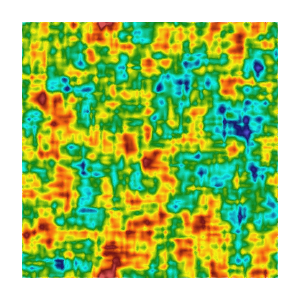
\includegraphics[width=\textwidth]{Chapter4/figures/2D/psic_exp_cartesian_5_5_rho_0_seed_d.png}
    \caption{}
    \label{fig: Chapter4/2D/psic_exp_cartesian_5_5_rho_0_seed_d}
  \end{subfigure}
  \begin{subfigure}[b]{0.15\textwidth}
    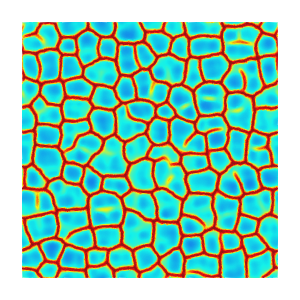
\includegraphics[width=\textwidth]{Chapter4/figures/2D/d_exp_cartesian_5_5_rho_0_seed_d.png}
    \caption{}
    \label{fig: Chapter4/2D/d_exp_cartesian_5_5_rho_0_seed_d}
  \end{subfigure}

  \begin{subfigure}[b]{0.15\textwidth}
    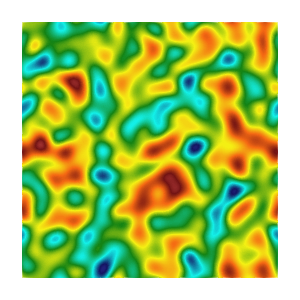
\includegraphics[width=\textwidth]{Chapter4/figures/2D/Gc_sqexp_cartesian_5_5_rho_0_seed_e.png}
    \caption{}
    \label{fig: Chapter4/2D/Gc_sqexp_cartesian_5_5_rho_0_seed_e}
  \end{subfigure}
  \begin{subfigure}[b]{0.15\textwidth}
    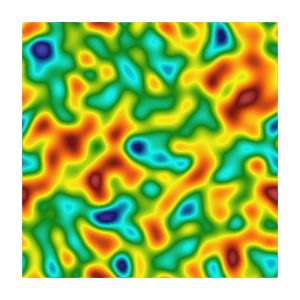
\includegraphics[width=\textwidth]{Chapter4/figures/2D/psic_sqexp_cartesian_5_5_rho_0_seed_e.png}
    \caption{}
    \label{fig: Chapter4/2D/psic_sqexp_cartesian_5_5_rho_0_seed_e}
  \end{subfigure}
  \begin{subfigure}[b]{0.15\textwidth}
    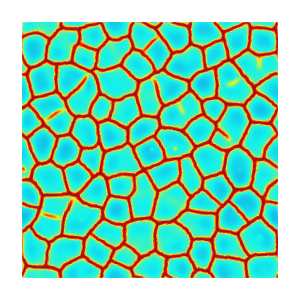
\includegraphics[width=\textwidth]{Chapter4/figures/2D/d_sqexp_cartesian_5_5_rho_0_seed_e.png}
    \caption{}
    \label{fig: Chapter4/2D/d_sqexp_cartesian_5_5_rho_0_seed_e}
  \end{subfigure}
  \begin{subfigure}[b]{0.15\textwidth}
    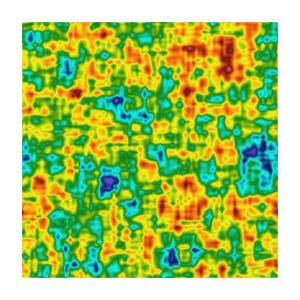
\includegraphics[width=\textwidth]{Chapter4/figures/2D/Gc_exp_cartesian_5_5_rho_0_seed_e.png}
    \caption{}
    \label{fig: Chapter4/2D/Gc_exp_cartesian_5_5_rho_0_seed_e}
  \end{subfigure}
  \begin{subfigure}[b]{0.15\textwidth}
    \includegraphics[width=\textwidth]{Chapter4/figures/2D/psic_exp_cartesian_5_5_rho_0_seed_e.png}
    \caption{}
    \label{fig: Chapter4/2D/psic_exp_cartesian_5_5_rho_0_seed_e}
  \end{subfigure}
  \begin{subfigure}[b]{0.15\textwidth}
    \includegraphics[width=\textwidth]{Chapter4/figures/2D/d_exp_cartesian_5_5_rho_0_seed_e.png}
    \caption{}
    \label{fig: Chapter4/2D/d_exp_cartesian_5_5_rho_0_seed_e}
  \end{subfigure}
  \caption{ Three pairs of qualitative comparison of smoothness of the kernel function with the same normalized  correlation length $L^* = 0.05$. (a-f) pair 1 (g-l) pair 2 (m-r) pair 3. Each row compares two kernel functions transformed from the same samples of the underlying Gaussian fields. }
  \label{fig: Chapter4/2D/compare_smoothness}
\end{figure}


\begin{figure}[htb!]
  \centering
  \begin{subfigure}[b]{0.475\textwidth}
    \centering
    \tikzsetnextfilenamesafe{Chapter4/2D/dimensionless_curve_smoothness}
    \begin{tikzpicture}
      \begin{axis}[
          width=\textwidth,
          height=0.9\textwidth,
          ymode=log,
          log ticks with fixed point,
          ylabel=$\underline{l^*}$,xlabel=$\mathcal{D}^*$,
          % ymin=0,ymax=2.5,
          legend style={
              at={(0.05,0.05)},
              anchor=south west,
              nodes={scale=1, transform shape},
              fill=none,
              draw=none,
              text opacity=1,
              cells={align=left}
            },
          legend cell align={left},
          every axis plot/.append style={thick}
        ]
        % sqexp
        \addplot [select coords between index={40}{220},color=black] table [x expr=\thisrowno{0},y expr=\thisrowno{1}]{Chapter4/data/2D/dimensionless_curve_sqexp_cartesian_5_5.csv};
        % exp
        \addplot [select coords between index={40}{220},color=red] table [x expr=\thisrowno{0},y expr=\thisrowno{1}]{Chapter4/data/2D/dimensionless_curve_exp_cartesian_5_5.csv};
        \legend{sqexp,exp}
      \end{axis}
    \end{tikzpicture}
    \caption{}
    \label{fig: Chapter4/2D/dimensionless_curve_smoothness}
  \end{subfigure}
  \begin{subfigure}[b]{0.475\textwidth}
    \centering
    \tikzsetnextfilenamesafe{hapter4/2D/distribution_smoothness}
    \begin{tikzpicture}
      \begin{axis}[
          width=\textwidth,
          height=0.9\textwidth,
          xlabel=$l^*$,ylabel=estimated PDF,
          ymin=0,ymax=0.012,
          xmin=0,xmax=300,
          legend style={at={(0.95,0.95)},anchor=north east},
          legend style={nodes={scale=1, transform shape}},
          legend style={fill=none, draw=none},
          legend cell align={left},
          every axis plot/.append style={thick}
        ]
        \addplot [color=black] table [x expr=\thisrowno{0},y expr=\thisrowno{1}]{Chapter4/data/2D/distribution_sqexp_cartesian_5_5.csv};
        \addplot [color=red] table [x expr=\thisrowno{0},y expr=\thisrowno{1}]{Chapter4/data/2D/distribution_exp_cartesian_5_5.csv};
        \legend{sqexp,exp}
      \end{axis}
    \end{tikzpicture}
    \caption{}
    \label{fig: Chapter4/2D/distribution_smoothness}
  \end{subfigure}
  \caption[Fragment statistics for different covariance kernels.]{Comparisons of (a) mean dimensionless crack spacing $\underline{l^*}$ versus dimensionless crack driving force $\mathcal{D}^*$ and (b) Estimated probability density of dimensionless crack spacing with the same correlation length when $\mathcal{D}^* = 5.17$ for results obtained using a PSE kernel and a PE kernel}
  \label{fig: Chapter4/2D/statistics_smoothness}
\end{figure}


Samples obtained with the two covariance models (parameterized by the same correlation lengths), considering the same realization for the underlying Gaussian field (from one covariance model to another), are compared in \Cref{fig: Chapter4/2D/compare_smoothness} to study the effect of smoothness. It is seen that rougher material properties provide more candidate locations for damage localization, hence resulting in more fragments per unit volume of the domain (in a statistical sense). More precisely, the probability density functions (PDFs) corresponding to the dimensionless crack spacing (\Cref{fig: Chapter4/2D/statistics_smoothness}), estimated using approximately 2000 fragments and 10 independent realizations of the fields, show a substantial difference:the mean fragment size obtained with rough material properties (here, with the PE model) turns out to be much smaller than the mean fragment size generated by smoother samples of fracture properties (associated with the PSE model).

%%%%%%%%%%%%%%%%%%%%%%%%%%%%%%%%%%%%%%%%%%%%%%%%%%%%%%%%%%%%%%%%%%%%%%%%%%%%%%%%%%%%%%%%%%%
%%%%%%%%%%%%%%%%%%%%%%%%%%%%%%%%%%%%%%%%%%%%%%%%%%%%%%%%%%%%%%%%%%%%%%%%%%%%%%%%%%%%%%%%%%%
%%%%%%%%%%%%%%%%%%%%%%%%%%%%%%%%%%%%%%%%%%%%%%%%%%%%%%%%%%%%%%%%%%%%%%%%%%%%%%%%%%%%%%%%%%%
%%%%%%%%%%%%%%%%%%%%%%%%%%%%%%%%%%%%%%%%%%%%%%%%%%%%%%%%%%%%%%%%%%%%%%%%%%%%%%%%%%%%%%%%%%%
%%%%%%%%%%%%%%%%%%%%%%%%%%%%%%%%%%%%%%%%%%%%%%%%%%%%%%%%%%%%%%%%%%%%%%%%%%%%%%%%%%%%%%%%%%%
%%%%%%%%%%%%%%%%%%%%%%%%%%%%%%%%%%%%%%%%%%%%%%%%%%%%%%%%%%%%%%%%%%%%%%%%%%%%%%%%%%%%%%%%%%%
%%%%%%%%%%%%%%%%%%%%%%%%%%%%%%%%%%%%%%%%%%%%%%%%%%%%%%%%%%%%%%%%%%%%%%%%%%%%%%%%%%%%%%%%%%%
%%%%%%%%%%%%%%%%%%%%%%%%%%%%%%%%%%%%%%%%%%%%%%%%%%%%%%%%%%%%%%%%%%%%%%%%%%%%%%%%%%%%%%%%%%%
%%%%%%%%%%%%%%%%%%%%%%%%%%%%%%%%%%%%%%%%%%%%%%%%%%%%%%%%%%%%%%%%%%%%%%%%%%%%%%%%%%%%%%%%%%%
%%%%%%%%%%%%%%%%%%%%%%%%%%%%%%%%%%%%%%%%%%%%%%%%%%%%%%%%%%%%%%%%%%%%%%%%%%%%%%%%%%%%%%%%%%%
\subsubsection{Parametric Analysis}

The stochastic model constructed in this paper enables the introduction of point-wise correlation (that is, in the first-order marginal probability distribution) between the two fracture properties.
With regard to fracture mechanics, one might wonder, for example, whether or not the fracture toughness $\Gc$ and the critical fracture energy $\psi_c$ are correlated (at a given location), and if so, to what extent. In this section, we perform a parametric analysis for different values of the correlation coefficient $\rho$, with the aim of understanding which field plays a dominant role in determining the resulting fracture morphology in thin films.

In order to obtain meaningful statistical results, 10 independent realizations are considered, and the same samples (of the underlying Gaussian random fields) are used when $\rho$ varies. The normalized correlation length is set to $L^* = 0.05$ for both fracture properties.
Three pairs of fracture toughness and critical fracture energy samples, constructed using \eqref{eq: def-P1} and \eqref{eq: def-P2} with $\rho \in \{0, 0.5, 1\}$, are shown in \Cref{fig: Chapter4/2D/compare_correlation}. Note that the special case of $\rho = 0$ recovers the case of independent material properties.

\begin{figure}[!htb]
  \centering
  \begin{subfigure}[b]{0.42\textwidth}
    \caption*{Squared Exponential Kernel}
  \end{subfigure}
  \begin{subfigure}[b]{0.42\textwidth}
    \caption*{Exponential Kernel}
  \end{subfigure}
  \hspace{0.05\textwidth}

  \begin{subfigure}[b]{0.14\textwidth}
    \caption*{$\rho = 0$}
  \end{subfigure}
  \begin{subfigure}[b]{0.14\textwidth}
    \caption*{$\rho = 0.5$}
  \end{subfigure}
  \begin{subfigure}[b]{0.14\textwidth}
    \caption*{$\rho = 1$}
  \end{subfigure}
  \begin{subfigure}[b]{0.14\textwidth}
    \caption*{$\rho = 0$}
  \end{subfigure}
  \begin{subfigure}[b]{0.14\textwidth}
    \caption*{$\rho = 0.5$}
  \end{subfigure}
  \begin{subfigure}[b]{0.14\textwidth}
    \caption*{$\rho = 1$}
  \end{subfigure}
  \hspace{0.05\textwidth}

  \begin{subfigure}[b]{0.14\textwidth}
    \includegraphics[width=\textwidth]{Chapter4/figures/2D/Gc_sqexp_cartesian_5_5_rho_1_sample_1.png}
    \caption{}
  \end{subfigure}
  \begin{subfigure}[b]{0.14\textwidth}
    \includegraphics[width=\textwidth]{Chapter4/figures/2D/Gc_sqexp_cartesian_5_5_rho_1_sample_1.png}
    \caption{}
  \end{subfigure}
  \begin{subfigure}[b]{0.14\textwidth}
    \includegraphics[width=\textwidth]{Chapter4/figures/2D/Gc_sqexp_cartesian_5_5_rho_1_sample_1.png}
    \caption{}
  \end{subfigure}
  \begin{subfigure}[b]{0.14\textwidth}
    \includegraphics[width=\textwidth]{Chapter4/figures/2D/Gc_exp_cartesian_5_5_rho_1_sample_1.png}
    \caption{}
  \end{subfigure}
  \begin{subfigure}[b]{0.14\textwidth}
    \includegraphics[width=\textwidth]{Chapter4/figures/2D/Gc_exp_cartesian_5_5_rho_1_sample_1.png}
    \caption{}
  \end{subfigure}
  \begin{subfigure}[b]{0.14\textwidth}
    \includegraphics[width=\textwidth]{Chapter4/figures/2D/Gc_exp_cartesian_5_5_rho_1_sample_1.png}
    \caption{}
  \end{subfigure}
  \begin{subfigure}[b]{0.05\textwidth}
    \caption*{$\Gc^*$}
    \includegraphics[width=\textwidth]{Chapter4/figures/rainbow_vertical.png}
    \vspace{0.05in}
  \end{subfigure}

  \begin{subfigure}[b]{0.14\textwidth}
    \includegraphics[width=\textwidth]{Chapter4/figures/2D/psic_sqexp_cartesian_5_5_rho_0_sample_1.png}
    \caption{}
  \end{subfigure}
  \begin{subfigure}[b]{0.14\textwidth}
    \includegraphics[width=\textwidth]{Chapter4/figures/2D/psic_sqexp_cartesian_5_5_rho_0_5_sample_1.png}
    \caption{}
  \end{subfigure}
  \begin{subfigure}[b]{0.14\textwidth}
    \includegraphics[width=\textwidth]{Chapter4/figures/2D/psic_sqexp_cartesian_5_5_rho_1_sample_1.png}
    \caption{}
  \end{subfigure}
  \begin{subfigure}[b]{0.14\textwidth}
    \includegraphics[width=\textwidth]{Chapter4/figures/2D/psic_exp_cartesian_5_5_rho_0_sample_1.png}
    \caption{}
  \end{subfigure}
  \begin{subfigure}[b]{0.14\textwidth}
    \includegraphics[width=\textwidth]{Chapter4/figures/2D/psic_exp_cartesian_5_5_rho_0_5_sample_1.png}
    \caption{}
  \end{subfigure}
  \begin{subfigure}[b]{0.14\textwidth}
    \includegraphics[width=\textwidth]{Chapter4/figures/2D/psic_exp_cartesian_5_5_rho_1_sample_1.png}
    \caption{}
  \end{subfigure}
  \begin{subfigure}[b]{0.05\textwidth}
    \caption*{$\psi_c^*$}
    \includegraphics[width=\textwidth]{Chapter4/figures/rainbow_vertical.png}
    \vspace{0.05in}
  \end{subfigure}
  \caption{ Point-wise correlated material properties: (a-f) normalized fracture toughness $\Gc^*$ and (g-l) normalized critical fracture energy $\psi_c^*$ with (left) PSE covariance function (right) PE covariance function }
  \label{fig: Chapter4/2D/compare_correlation}
\end{figure}


Statistics of the dimensionless crack spacing $l^*$ are once again extracted at $\mathcal{D}^* = 5.17$. The resulting dimensionless curves and normalized probability density functions are shown in \Cref{fig: Chapter4/2D/statistics_sensitivity_sqexp,fig: Chapter4/2D/statistics_sensitivity_exp}. These results indicate that the distribution of fragment size is relatively insensitive to the coefficient of correlation, regardless of the smoothness of the covariance kernel.

\begin{figure}[htb!]
  \centering
  \begin{subfigure}[b]{0.475\textwidth}
    \centering
    \tikzsetnextfilenamesafe{Chapter4/2D/statistics_sensitivity_sqexp/dimensionless_curve}
    \begin{tikzpicture}
      \begin{axis}[
          width=\textwidth,
          height=0.9\textwidth,
          ymode=log,
          log ticks with fixed point,
          ylabel=$\underline{l^*}$,xlabel=$\mathcal{D}^*$,
          % ymin=0,ymax=2.5,
          legend style={
              at={(0.05,0.05)},
              anchor=south west,
              nodes={scale=1, transform shape},
              fill=white,
              fill opacity=0.8,
              draw opacity=1,
              text opacity=1,
              cells={align=left}
            },
          legend cell align={left},
          every axis plot/.append style={thick}
        ]
        % rho = 0
        \addplot [select coords between index={40}{220},color=black] table [x expr=\thisrowno{0},y expr=\thisrowno{1}]{Chapter4/data/2D/dimensionless_curve_sqexp_rho_1.csv};
        % rho = 0.5
        \addplot [select coords between index={40}{220},color=red] table [x expr=\thisrowno{0},y expr=\thisrowno{1}]{Chapter4/data/2D/dimensionless_curve_sqexp_rho_2.csv};
        % rho = 1
        \addplot [select coords between index={40}{220},color=blue] table [x expr=\thisrowno{0},y expr=\thisrowno{1}]{Chapter4/data/2D/dimensionless_curve_sqexp_rho_3.csv};
        \legend{$\rho=0$,$\rho=0.5$,$\rho=1$}
      \end{axis}
    \end{tikzpicture}
    \caption{}
  \end{subfigure}
  \begin{subfigure}[b]{0.475\textwidth}
    \centering
    \tikzsetnextfilenamesafe{Chapter4/2D/statistics_sensitivity_sqexp/distribution}
    \begin{tikzpicture}
      \begin{axis}[
          width=\textwidth,
          height=0.9\textwidth,
          xlabel=$l^*$,ylabel=estimated PDF,
          ymin=0,ymax=0.012,
          xmin=0,xmax=300,
          legend style={at={(0.95,0.95)},anchor=north east},
          legend style={nodes={scale=1, transform shape}},
          legend cell align={left},
          every axis plot/.append style={thick}
        ]
        \addplot [color=black] table [x expr=\thisrowno{0},y expr=\thisrowno{1}]{Chapter4/data/2D/distribution_sqexp_rho_1.csv};
        \addplot [color=red] table [x expr=\thisrowno{0},y expr=\thisrowno{1}]{Chapter4/data/2D/distribution_sqexp_rho_2.csv};
        \addplot [color=blue] table [x expr=\thisrowno{0},y expr=\thisrowno{1}]{Chapter4/data/2D/distribution_sqexp_rho_3.csv};
        \legend{$\rho=0$,$\rho=0.5$,$\rho=1$}
      \end{axis}
    \end{tikzpicture}
    \caption{}
  \end{subfigure}
  \caption{Comparisons of (a) mean dimensionless crack spacing as a function of dimensionless crack driving force and (b) estimated PDFs of dimensionless fragment size at loading $\mathcal{D}^* = 5.17$ for results with an underlying PSE kernel}
  \label{fig: Chapter4/2D/statistics_sensitivity_sqexp}
\end{figure}

\begin{figure}[htb!]
  \centering
  \begin{subfigure}[b]{0.475\textwidth}
    \centering
    \tikzsetnextfilenamesafe{Chapter4/2D/statistics_sensitivity_exp/dimensionless_curve}
    \begin{tikzpicture}
      \begin{axis}[
          width=\textwidth,
          height=0.9\textwidth,
          ymode=log,
          log ticks with fixed point,
          ylabel=$\underline{l^*}$,xlabel=$\mathcal{D}^*$,
          % ymin=0,ymax=2.5,
          legend style={
              at={(0.05,0.05)},
              anchor=south west,
              nodes={scale=1, transform shape},
              fill=white,
              fill opacity=0.8,
              draw opacity=1,
              text opacity=1,
              cells={align=left}
            },
          legend cell align={left},
          every axis plot/.append style={thick}
        ]
        % rho = 0
        \addplot [select coords between index={40}{220},color=black] table [x expr=\thisrowno{0},y expr=\thisrowno{1}]{Chapter4/data/2D/dimensionless_curve_exp_rho_1.csv};
        % rho = 0.5
        \addplot [select coords between index={40}{220},color=red] table [x expr=\thisrowno{0},y expr=\thisrowno{1}]{Chapter4/data/2D/dimensionless_curve_exp_rho_2.csv};
        % rho = 1
        \addplot [select coords between index={40}{220},color=blue] table [x expr=\thisrowno{0},y expr=\thisrowno{1}]{Chapter4/data/2D/dimensionless_curve_exp_rho_3.csv};
        \legend{$\rho=0$,$\rho=0.5$,$\rho=1$}
      \end{axis}
    \end{tikzpicture}
    \caption{}
  \end{subfigure}
  \begin{subfigure}[b]{0.475\textwidth}
    \centering
    \tikzsetnextfilenamesafe{Chapter4/2D/statistics_sensitivity_exp/distribution}
    \begin{tikzpicture}
      \begin{axis}[
          width=\textwidth,
          height=0.9\textwidth,
          xlabel=$l^*$,ylabel=estimated PDF,
          ymin=0,ymax=0.012,
          xmin=0,xmax=300,
          legend style={at={(0.95,0.95)},anchor=north east},
          legend style={nodes={scale=1, transform shape}},
          legend cell align={left},
          every axis plot/.append style={thick}
        ]
        \addplot [color=black] table [x expr=\thisrowno{0},y expr=\thisrowno{1}]{Chapter4/data/2D/distribution_exp_rho_1.csv};
        \addplot [color=red] table [x expr=\thisrowno{0},y expr=\thisrowno{1}]{Chapter4/data/2D/distribution_exp_rho_2.csv};
        \addplot [color=blue] table [x expr=\thisrowno{0},y expr=\thisrowno{1}]{Chapter4/data/2D/distribution_exp_rho_3.csv};
        \legend{$\rho=0$,$\rho=0.5$,$\rho=1$}
      \end{axis}
    \end{tikzpicture}
    \caption{}
  \end{subfigure}
  \caption{Comparisons of (a) mean dimensionless crack spacing and dimensionless crack driving force and (b) estimated PDFs of dimensionless fragment size at loading $\mathcal{D}^* = 5.17$ for results with an underlying PE kernel}
  \label{fig: Chapter4/2D/statistics_sensitivity_exp}
\end{figure}


In contrast, when we superimpose the fracture patterns, we observe that the fracture morphology does exhibit a sensitivity to variations in the fracture toughness  (\Cref{fig: Chapter4/2D/morphology_psic_constant}). The superimposed results are only shown for the PSE covariance function, but comparable results are obtained with the PE covariance function.
By comparison, when the fracture toughness is held fixed while the critical fracture energy is varied, the superimposed fracture patterns are nearly indistinguishable (\Cref{fig: Chapter4/2D/morphology_Gc_constant}). The clear conclusion is that the energetics are primarily responsible for driving the fracture morphology, a result that is not surprising. This conclusion is also supported by the results shown in \Cref{fig: Chapter4/2D/compare_sensitivity_sqexp,fig: Chapter4/2D/compare_sensitivity_exp}, in which fracture patterns are plotted over contours of the fracture toughness and the critical energy. For both types of covariance functions, the fracture patterns are seen to follow contours of minimal fracture toughness while largely ignoring those of the critical fracture energy.

% !TEX root = ../../../main.tex

\begin{figure}[!htbp]
  \centering
  \begin{subfigure}[b]{0.4\textwidth}
    \includegraphics[width=\textwidth]{Chapter4/figures/2D/psic_constant.png}
    \caption{}
    \label{fig: Chapter4/2D/morphology_psic_constant}
  \end{subfigure}
  \begin{subfigure}[b]{0.4\textwidth}
    \includegraphics[width=\textwidth]{Chapter4/figures/2D/Gc_constant.png}
    \caption{}
    \label{fig: Chapter4/2D/morphology_Gc_constant}
  \end{subfigure}
  \begin{subfigure}[b]{0.1\textwidth}
    \includegraphics[width=\textwidth]{Chapter4/figures/rho.png}
    \caption*{}
    \vspace{0.75in}
  \end{subfigure}
  \caption[Superposition of fracture networks obtained by three samples of different coefficients of correlation, using the PSE kernel.]{ Superposition of fracture networks obtained by three samples of different coefficients of correlation, using the PSE kernel. Only the volume within the damage contour of $d = 0.9$ is shown to represent the resulting fracture network. Three samples are sampled (a) by holding $\Gc$ constant and (b) by holding $\psi_c$ constant. }
  \label{fig: Chapter4/2D/compare_morphology}
\end{figure}


\begin{figure}[!htbp]
  \centering
  \begin{subfigure}[b]{0.25\textwidth}
    \includegraphics[width=\textwidth]{Chapter4/figures/2D/Gc_sqexp_cartesian_5_5_rho_0_seed_a_with_crack_140.png}
    \caption{$\mathcal{D}^* = 3.06$}
    \label{fig: Chapter4/2D/Gc_sqexp_cartesian_5_5_rho_0_seed_a_with_crack_140}
  \end{subfigure}
  \begin{subfigure}[b]{0.25\textwidth}
    \includegraphics[width=\textwidth]{Chapter4/figures/2D/Gc_sqexp_cartesian_5_5_rho_0_seed_a_with_crack_160.png}
    \caption{$\mathcal{D}^* = 3.76$}
    \label{fig: Chapter4/2D/Gc_sqexp_cartesian_5_5_rho_0_seed_a_with_crack_160}
  \end{subfigure}
  \begin{subfigure}[b]{0.25\textwidth}
    \includegraphics[width=\textwidth]{Chapter4/figures/2D/Gc_sqexp_cartesian_5_5_rho_0_seed_a_with_crack_220.png}
    \caption{$\mathcal{D}^* = 5.17$}
    \label{fig: Chapter4/2D/Gc_sqexp_cartesian_5_5_rho_0_seed_a_with_crack_220}
  \end{subfigure}
  \begin{subfigure}[b]{0.08\textwidth}
    \caption*{$\Gc^*$}
    \includegraphics[width=\textwidth]{Chapter4/figures/rainbow_vertical.png}
    \vspace{0.15in}
  \end{subfigure}
  
  \begin{subfigure}[b]{0.25\textwidth}
    \includegraphics[width=\textwidth]{Chapter4/figures/2D/psic_sqexp_cartesian_5_5_rho_0_seed_a_with_crack_140.png}
    \caption{$\mathcal{D}^* = 3.06$}
    \label{fig: Chapter4/2D/psic_sqexp_cartesian_5_5_rho_0_seed_a_with_crack_140}
  \end{subfigure}
  \begin{subfigure}[b]{0.25\textwidth}
    \includegraphics[width=\textwidth]{Chapter4/figures/2D/psic_sqexp_cartesian_5_5_rho_0_seed_a_with_crack_160.png}
    \caption{$\mathcal{D}^* = 3.76$}
    \label{fig: Chapter4/2D/psic_sqexp_cartesian_5_5_rho_0_seed_a_with_crack_160}
  \end{subfigure}
  \begin{subfigure}[b]{0.25\textwidth}
    \includegraphics[width=\textwidth]{Chapter4/figures/2D/psic_sqexp_cartesian_5_5_rho_0_seed_a_with_crack_220.png}
    \caption{$\mathcal{D}^* = 5.17$}
    \label{fig: Chapter4/2D/psic_sqexp_cartesian_5_5_rho_0_seed_a_with_crack_220}
  \end{subfigure}
  \begin{subfigure}[b]{0.08\textwidth}
    \caption*{$\psi_c^*$}
    \includegraphics[width=\textwidth]{Chapter4/figures/rainbow_vertical.png}
    \vspace{0.15in}
  \end{subfigure}
  \caption[Snapshots of phase field at different loading levels with a PSE covariance function.]{Snapshots of phase field at different loading levels with $d \geqslant 0.75$ plotted over (a-c) fracture toughness $\Gc$ and (d-f) critical fracture energy $\psi_c$ with an underlying PSE covariance function }
  \label{fig: Chapter4/2D/compare_sensitivity_sqexp}
\end{figure}

\begin{figure}[!htbp]
  \centering
  \begin{subfigure}[b]{0.25\textwidth}
    \includegraphics[width=\textwidth]{Chapter4/figures/2D/Gc_exp_cartesian_5_5_rho_0_seed_b_with_crack_140.png}
    \caption{$\mathcal{D}^* = 3.06$}
    \label{fig: Chapter4/2D/Gc_exp_cartesian_5_5_rho_0_seed_a_with_crack_140}
  \end{subfigure}
  \begin{subfigure}[b]{0.25\textwidth}
    \includegraphics[width=\textwidth]{Chapter4/figures/2D/Gc_exp_cartesian_5_5_rho_0_seed_b_with_crack_160.png}
    \caption{$\mathcal{D}^* = 3.76$}
    \label{fig: Chapter4/2D/Gc_exp_cartesian_5_5_rho_0_seed_a_with_crack_160}
  \end{subfigure}
  \begin{subfigure}[b]{0.25\textwidth}
    \includegraphics[width=\textwidth]{Chapter4/figures/2D/Gc_exp_cartesian_5_5_rho_0_seed_b_with_crack_220.png}
    \caption{$\mathcal{D}^* = 5.17$}
    \label{fig: Chapter4/2D/Gc_exp_cartesian_5_5_rho_0_seed_a_with_crack_220}
  \end{subfigure}
  \begin{subfigure}[b]{0.08\textwidth}
    \caption*{$\Gc^*$}
    \includegraphics[width=\textwidth]{Chapter4/figures/rainbow_vertical.png}
    \vspace{0.15in}
  \end{subfigure}
  
  \begin{subfigure}[b]{0.25\textwidth}
    \includegraphics[width=\textwidth]{Chapter4/figures/2D/psic_exp_cartesian_5_5_rho_0_seed_b_with_crack_140.png}
    \caption{$\mathcal{D}^* = 3.06$}
    \label{fig: Chapter4/2D/psic_exp_cartesian_5_5_rho_0_seed_a_with_crack_140}
  \end{subfigure}
  \begin{subfigure}[b]{0.25\textwidth}
    \includegraphics[width=\textwidth]{Chapter4/figures/2D/psic_exp_cartesian_5_5_rho_0_seed_b_with_crack_160.png}
    \caption{$\mathcal{D}^* = 3.76$}
    \label{fig: Chapter4/2D/psic_exp_cartesian_5_5_rho_0_seed_a_with_crack_160}
  \end{subfigure}
  \begin{subfigure}[b]{0.25\textwidth}
    \includegraphics[width=\textwidth]{Chapter4/figures/2D/psic_exp_cartesian_5_5_rho_0_seed_b_with_crack_220.png}
    \caption{$\mathcal{D}^* = 5.17$}
    \label{fig: Chapter4/2D/psic_exp_cartesian_5_5_rho_0_seed_a_with_crack_220}
  \end{subfigure}
  \begin{subfigure}[b]{0.08\textwidth}
    \caption*{$\psi_c^*$}
    \includegraphics[width=\textwidth]{Chapter4/figures/rainbow_vertical.png}
    \vspace{0.15in}
  \end{subfigure}
  \caption[Snapshots of phase field at different loading levels with a PE covariance function.]{Snapshots of phase field at different loading levels with $d \geqslant 0.75$ plotted over (a-c) fracture toughness $\Gc$ and (d-f) critical fracture energy $\psi_c$ with an underlying PE covariance function }
  \label{fig: Chapter4/2D/compare_sensitivity_exp}
\end{figure}


%%%%%%%%%%%%%%%%%%%%%%%%%%%%%%%%%%%%%%%%%%%%%%%%%%%%%%%%%%%%%%%%%%%%%%%%%%%%%%%%%%%%%%%%%%%
%%%%%%%%%%%%%%%%%%%%%%%%%%%%%%%%%%%%%%%%%%%%%%%%%%%%%%%%%%%%%%%%%%%%%%%%%%%%%%%%%%%%%%%%%%%
%%%%%%%%%%%%%%%%%%%%%%%%%%%%%%%%%%%%%%%%%%%%%%%%%%%%%%%%%%%%%%%%%%%%%%%%%%%%%%%%%%%%%%%%%%%
%%%%%%%%%%%%%%%%%%%%%%%%%%%%%%%%%%%%%%%%%%%%%%%%%%%%%%%%%%%%%%%%%%%%%%%%%%%%%%%%%%%%%%%%%%%
%%%%%%%%%%%%%%%%%%%%%%%%%%%%%%%%%%%%%%%%%%%%%%%%%%%%%%%%%%%%%%%%%%%%%%%%%%%%%%%%%%%%%%%%%%%
%%%%%%%%%%%%%%%%%%%%%%%%%%%%%%%%%%%%%%%%%%%%%%%%%%%%%%%%%%%%%%%%%%%%%%%%%%%%%%%%%%%%%%%%%%%
%%%%%%%%%%%%%%%%%%%%%%%%%%%%%%%%%%%%%%%%%%%%%%%%%%%%%%%%%%%%%%%%%%%%%%%%%%%%%%%%%%%%%%%%%%%
%%%%%%%%%%%%%%%%%%%%%%%%%%%%%%%%%%%%%%%%%%%%%%%%%%%%%%%%%%%%%%%%%%%%%%%%%%%%%%%%%%%%%%%%%%%
%%%%%%%%%%%%%%%%%%%%%%%%%%%%%%%%%%%%%%%%%%%%%%%%%%%%%%%%%%%%%%%%%%%%%%%%%%%%%%%%%%%%%%%%%%%
%%%%%%%%%%%%%%%%%%%%%%%%%%%%%%%%%%%%%%%%%%%%%%%%%%%%%%%%%%%%%%%%%%%%%%%%%%%%%%%%%%%%%%%%%%%
\subsubsection{Discussion on Modeling Flexibility: Impact of the Covariance Structure}

We now briefly examine how different structures of the covariance kernel can alter the fragment morphology. It has been demonstrated experimentally \cite{kitsunezaki2016shaking, kitsunezaki2017stress, halasz2017effect, kitsunezaki2017memory, nakahara2018mechanism}
how macro-scale processing conditions to construct samples may lead to morphologically different crack networks.  For example, \citet{kitsunezaki2017memory} carried out a series of tests to study the effect of macroscopic disturbances on crack patterns. They poured calcium carbonate (CaCO$_3$) paste into a shallow circular container. Different modes of agitation were applied to the paste before it was dried, and the resulting crack patterns showed a strong correlation with the modes of agitation.

We hypothesize that the agitation gives rise to effective fracture properties at the macro-scale that have a structure that is consistent with the agitation. We further assume a rougher spatial variation of properties in the direction parallel to the agitation than in the direction orthogonal to the agitation. Accordingly, we model the spatial variations in the fracture properties using composite covariance functions, defined on purpose by a tensor-product structure involving PSE and PE functions. In Figure \ref{fig: Chapter4/2D/japanese_experiments}, we compare the experimentally-observed crack patterns to our simulation results obtained using random fracture properties with the postulated anisotropic covariance functions. The comparison shows reasonable agreement (without specifically optimizing the  hyperparameters in the stochastic model), indicating that the differing processing conditions may have resulted in different spatial variations in the effective fracture properties.

\begin{figure}[htb!]
  \centering
  \begin{subfigure}{0.14\textwidth}
    \caption*{Mode of agitation}
  \end{subfigure}
  \hspace{0.02\textwidth}
  \begin{subfigure}{0.14\textwidth}
    \caption*{\protect\raggedright Experimental crack network}
  \end{subfigure}
  \hspace{0.02\textwidth}
  \begin{subfigure}{0.15\textwidth}
    \caption*{$\Gc^*$}
    \includegraphics[width=\textwidth]{Chapter4/figures/rainbow_horizontal.png}
  \end{subfigure}
  \begin{subfigure}{0.15\textwidth}
    \caption*{$\psi_c^*$}
    \includegraphics[width=\textwidth]{Chapter4/figures/rainbow_horizontal.png}
  \end{subfigure}
  \begin{subfigure}{0.15\textwidth}
    \caption*{$d$}
    \includegraphics[width=\textwidth]{Chapter4/figures/grayscale_horizontal.png}
  \end{subfigure}
  
  \begin{subfigure}{0.14\textwidth}
    \includegraphics[width=\textwidth]{Chapter4/figures/2D/brick_schematic.png}
    \caption{}
  \end{subfigure}
  \hspace{0.02\textwidth}
  \begin{subfigure}{0.14\textwidth}
    \includegraphics[width=\textwidth]{Chapter4/figures/2D/paste_brick.png}
    \caption{}
  \end{subfigure}
  \hspace{0.02\textwidth}
  \begin{subfigure}{0.15\textwidth}
    \includegraphics[width=\textwidth]{Chapter4/figures/2D/Gc_brick.png}
    \caption{}
  \end{subfigure}
  \begin{subfigure}{0.15\textwidth}
    \includegraphics[width=\textwidth]{Chapter4/figures/2D/psic_brick.png}
    \caption{}
  \end{subfigure}
  \begin{subfigure}{0.15\textwidth}
    \includegraphics[width=\textwidth]{Chapter4/figures/2D/d_brick.png}
    \caption{}
  \end{subfigure}
  
  \begin{subfigure}{0.14\textwidth}
    \includegraphics[width=\textwidth]{Chapter4/figures/2D/radial_schematic.png}
    \caption{}
  \end{subfigure}
  \hspace{0.02\textwidth}
  \begin{subfigure}{0.14\textwidth}
    \includegraphics[width=\textwidth]{Chapter4/figures/2D/paste_radial.png}
    \caption{}
  \end{subfigure}
  \hspace{0.02\textwidth}
  \begin{subfigure}{0.15\textwidth}
    \includegraphics[width=\textwidth]{Chapter4/figures/2D/Gc_radial.png}
    \caption{}
  \end{subfigure}
  \begin{subfigure}{0.15\textwidth}
    \includegraphics[width=\textwidth]{Chapter4/figures/2D/psic_radial.png}
    \caption{}
  \end{subfigure}
  \begin{subfigure}{0.15\textwidth}
    \includegraphics[width=\textwidth]{Chapter4/figures/2D/d_radial.png}
    \caption{}
  \end{subfigure}
  
  \begin{subfigure}{0.14\textwidth}
    \includegraphics[width=\textwidth]{Chapter4/figures/2D/ring_schematic.png}
    \caption{}
  \end{subfigure}
  \hspace{0.02\textwidth}
  \begin{subfigure}{0.14\textwidth}
    \includegraphics[width=\textwidth]{Chapter4/figures/2D/paste_ring.png}
    \caption{}
  \end{subfigure}
  \hspace{0.02\textwidth}
  \begin{subfigure}{0.15\textwidth}
    \includegraphics[width=\textwidth]{Chapter4/figures/2D/Gc_ring.png}
    \caption{}
  \end{subfigure}
  \begin{subfigure}{0.15\textwidth}
    \includegraphics[width=\textwidth]{Chapter4/figures/2D/psic_ring.png}
    \caption{}
  \end{subfigure}
  \begin{subfigure}{0.15\textwidth}
    \includegraphics[width=\textwidth]{Chapter4/figures/2D/d_ring.png}
    \caption{}
  \end{subfigure}
  \caption[Three sets of experiments and calculations with different modes of agitation.]{Three sets of experiments and calculations for (a-e) unilateral agitation (f-j) rotational agitation (k-o) point agitation. (b, g, l) snapshots of crack patterns from experiments. postulated spatially correlated (c, h, m) fracture toughness and (d, i, n) critical fracture energy to reproduce experimental observations. (e, j, o) phase fields obtained using corresponding spatially varying material properties. }
  \label{fig: Chapter4/2D/japanese_experiments}
\end{figure}


%%%%%%%%%%%%%%%%%%%%%%%%%%%%%%%%%%%%%%%%%%%%%%%%%%%%%%%%%%%%%%%%%%%%%%%%%%%%%%%%%%%%%%%%%%%
%%%%%%%%%%%%%%%%%%%%%%%%%%%%%%%%%%%%%%%%%%%%%%%%%%%%%%%%%%%%%%%%%%%%%%%%%%%%%%%%%%%%%%%%%%%
%%%%%%%%%%%%%%%%%%%%%%%%%%%%%%%%%%%%%%%%%%%%%%%%%%%%%%%%%%%%%%%%%%%%%%%%%%%%%%%%%%%%%%%%%%%
%%%%%%%%%%%%%%%%%%%%%%%%%%%%%%%%%%%%%%%%%%%%%%%%%%%%%%%%%%%%%%%%%%%%%%%%%%%%%%%%%%%%%%%%%%%
%%%%%%%%%%%%%%%%%%%%%%%%%%%%%%%%%%%%%%%%%%%%%%%%%%%%%%%%%%%%%%%%%%%%%%%%%%%%%%%%%%%%%%%%%%%
%%%%%%%%%%%%%%%%%%%%%%%%%%%%%%%%%%%%%%%%%%%%%%%%%%%%%%%%%%%%%%%%%%%%%%%%%%%%%%%%%%%%%%%%%%%
%%%%%%%%%%%%%%%%%%%%%%%%%%%%%%%%%%%%%%%%%%%%%%%%%%%%%%%%%%%%%%%%%%%%%%%%%%%%%%%%%%%%%%%%%%%
%%%%%%%%%%%%%%%%%%%%%%%%%%%%%%%%%%%%%%%%%%%%%%%%%%%%%%%%%%%%%%%%%%%%%%%%%%%%%%%%%%%%%%%%%%%
%%%%%%%%%%%%%%%%%%%%%%%%%%%%%%%%%%%%%%%%%%%%%%%%%%%%%%%%%%%%%%%%%%%%%%%%%%%%%%%%%%%%%%%%%%%
%%%%%%%%%%%%%%%%%%%%%%%%%%%%%%%%%%%%%%%%%%%%%%%%%%%%%%%%%%%%%%%%%%%%%%%%%%%%%%%%%%%%%%%%%%%
\subsection{Inverse Identification Based on Three-Dimensional Physical Experiments}
\label{section: Chapter4/examples/3D}

In \citet{Rodriguez2006}, a series of drying tests with mining waste placed on grooved circular plates (\SI{225}{\milli\meter} in diameter) was performed to observe crack evolution due to desiccation processes. Three tests were carried out with different film thicknesses $h \in \{ \SI{4}{\milli\meter}, \SI{8}{\milli\meter}, \text{and}~\SI{16}{\milli\meter} \}$.

\begin{table}[htb!]
  \centering
  \caption{Summary of material properties of mining waste and model parameters for all calculations in \Cref{section: Chapter4/examples/3D}}
  \begin{tabular}{r c c c c}
    \toprule
    Property/Parameter            & Symbol                      & Value & Unit                                & Comment                                                     \\
    \midrule
    Young's modulus               & $E$                         & 4     & \SI{}{\mega\pascal}                 & See \cite{sanchez2014modeling}                              \\
    Poisson's ratio               & $\nu$                       & 0.2   & nondim.                             & See \cite{sanchez2014modeling}                              \\
    Mean fracture toughness       & $\underline{\mathcal{G}_c}$ & 27    & \SI{}{\kilo\joule\per\square\meter} & See \cite{rodriguez2007experimental,lakshmikantha2009image} \\[5pt]
    Mean critical fracture energy & $\underline{\psi_c}$        & 30    & \SI{}{\joule\per\square\meter}      & See \cite{rodriguez2007experimental,lakshmikantha2009image} \\[5pt]
    Regularization length         & $l$                         & 0.8   & \SI{}{\milli\meter}                 & Such that $2l/h^e \approx 5$                                \\
    Degradation shape parameter   & $p$                         & 1     & nondim.                             &                                                             \\
    \bottomrule
  \end{tabular}
  \label{tab: MW}
\end{table}

\begin{figure}
  \centering
  \begin{overpic}[scale=0.55]{Chapter4/figures/3D/inverse.png}
    \put(4,-4){\footnotesize\textbf{(a)}}
    \put(32,-4){\footnotesize\textbf{(b)}}
    \put(57,-4){\footnotesize\textbf{(c)}}
    \put(89,-4){\footnotesize\textbf{(d)}}
  \end{overpic}
  \vspace{0.2in}
  \caption[Procedures of finding the optimal hyperparameter to match the experiment.]{Procedures of finding the optimal hyperparameter to match the experiment: (a)  12 pairs of fracture properties are sampled to explore the space of admissible spatial correlation lengths; three dimensional energy minimization problems are solved to obtain (b) the resulting fracture morphology; (c) distributions of fragment sizes are extracted from the simulated results, and the log-likelihood values of these distributions at the samples extracted from (d) the experimental fracture morphology are computed.}
  \label{fig: Chapter4/3D/inverse}
\end{figure}


To replicate this study using model-based simulations and our phase-field model (enhanced with the stochastic description of fracture properties), we adopt fully three-dimensional models.  The material properties used for this study are  listed in \Cref{tab: MW}.  Consistent with the experimental studies of \cite{Rodriguez2006}, the film-substrate system is represented by a cylindrical domain. The substrate is modeled as a rigid body with an arbitrarily high fracture toughness. The substrate and film are discretized using tetrahedral elements with characteristic lengths of $h^e_0 = \SI{1.6}{\milli\meter}$ and $h^e_1 = \SI{0.36}{\milli\meter}$, respectively. The solutions to the linear elasticity subproblem, the fracture subproblem, and the generalized eigenvalue problem are once again approximated using the same mesh.

We first calibrate the spatial variability in our model against the experimental observations of the fracture patterns for the thinnest ($h = 4$mm) specimen. To formulate the statistical inverse problem, we assume that (1) the fracture toughness and the critical fracture energy are uncorrelated (i.e., $\rho = 0$); and (2) both fracture properties have the same coefficient of variation (set to 0.03) and spatial correlation lengths, and that they can be defined using isotropic squared exponential kernels. In addition, the variations of the properties through the thickness of the film are assumed negligible compared to in-plane variations.

Based on these assumptions, the spatial correlation length $L$ is the only parameter to be determined, and a parametric search is performed in $\mathbb{L} = \{$ \SI{3}{\milli\meter}, \SI{3.5}{\milli\meter}, \SI{4}{\milli\meter}, \SI{4.5}{\milli\meter}, \SI{5}{\milli\meter}, \SI{5.5}{\milli\meter}, \SI{6}{\milli\meter}, \SI{6.5}{\milli\meter}, \SI{7}{\milli\meter}, \SI{7.5}{\milli\meter}, \SI{8}{\milli\meter}, \SI{8.5}{\milli\meter} $\}$. Energy minimization problems for the case of $h = \SI{4}{\milli\meter}$ are simulated for each pair of realizations and the corresponding fracture patterns are obtained. For a given value of $L \in \mathbb{L}$, the flooding algorithm is used to identify fragments on the top surface of the thin film, and a kernel density estimation of the probability density function associated with the fragment size, denoted by $f_\text{fs}^\text{sim}(\cdot; L)$, is obtained. The optimal value of $L$ is then identified by maximizing the log-likelihood function $\mathcal{L}$ defined as
\begin{align}
  \mathcal{L}(L) = \sum_{A_\text{fs}^\text{exp} \in \mathbb{A}^\text{exp}} \ln{f_\text{fs}^\text{sim}(l^*(A_\text{fs}^\text{exp}); L)}~, \quad l^*(A) = \dfrac{\sqrt{A}}{h}~,
\end{align}
where $\mathbb{A}^\text{exp}$ denotes the collection of fragment size samples extracted by using the same flooding algorithm on the experimental result.
The aforementioned workflow to calibrate the model is summarized in \Cref{fig: Chapter4/3D/inverse}. The fracture properties with spatial correlation $L = \SI{4}{\milli\meter}$ lead to the maximum log-likelihood among the span of samples considered. \Cref{fig: Chapter4/3D/calibrated} compares the estimated PDF and the fracture morphology obtained using the calibrated stochastic model to those of the experimental specimen for $h = \SI{4}{\milli\meter}$.

\begin{figure}[!htbp]
  \centering
  \begin{subfigure}[b]{0.4\textwidth}
    \centering
    \tikzsetnextfilenamesafe{Chapter4/3D/calibrated/pdf}
    \begin{tikzpicture}
      \begin{axis}[
          width=\textwidth,
          height=1\textwidth,
          xlabel=$l^*$,ylabel=estimated PDF,
          ymin=0,ymax=0.5,
          xmin=0,xmax=15,
          legend style={at={(0.95,0.95)},anchor=north east},
          legend style={nodes={scale=1, transform shape}},
          legend style={fill=none, draw=none},
          legend cell align={left},
          every axis plot/.append style={thick}
        ]
        \addplot [color=black] table [x expr=\thisrowno{0},y expr=\thisrowno{1}]{Chapter4/data/3D/calibrated_pdf.csv};
        \addplot [color=red] table [x expr=\thisrowno{0},y expr=\thisrowno{2}]{Chapter4/data/3D/calibrated_pdf.csv};
        \legend{experiment,simulation}
      \end{axis}
    \end{tikzpicture}
    \caption{}
  \end{subfigure}
  \begin{subfigure}[b]{0.27\textwidth}
    \centering
    \includegraphics[width=\textwidth]{Chapter4/figures/3D/d_4.png}
    \vspace{10pt}
    \caption{}
  \end{subfigure}
  \begin{subfigure}[b]{0.25\textwidth}
    \centering
    \includegraphics[width=\textwidth]{Chapter4/figures/3D/4mm_exp.png}
    \vspace{12pt}
    \caption{}
  \end{subfigure}
  \caption{(a) Estimated PDFs of the dimensionless fragment sizes extracted from the experimental result and the calibrated stochastic model. (b) Fracture morphology obtained using the calibrated fracture properties. (c) Photograph of cracks in the mining waste. }
  \label{fig: Chapter4/3D/calibrated}
\end{figure}


To then benchmark our model against specimens with different thicknesses, three 3D calculations are carried out using the same realization of fracture properties with $L = \SI{4}{\milli\meter}$. As shown in \Cref{fig: Chapter4/3D/3D},
our results appear to agree reasonably well with the experimental observations. In general, the thicker films fracture into larger fragments, which also agrees with the simplified models presented in \Cref{section: Chapter4/examples/1D,section: Chapter4/examples/2D}.

\begin{figure}[!htb]
  \centering
  \begin{subfigure}{0.23\textwidth}
    \includegraphics[width=\textwidth,scale=0.5]{Chapter4/figures/3D/4mm_exp.png}
    \caption{}
  \end{subfigure}
  \hspace{0.05\textwidth}
  \begin{subfigure}{0.23\textwidth}
    \includegraphics[width=\textwidth,scale=0.5]{Chapter4/figures/3D/8mm_exp.png}
    \caption{}
  \end{subfigure}
  \hspace{0.05\textwidth}
  \begin{subfigure}{0.23\textwidth}
    \includegraphics[width=\textwidth,scale=0.5]{Chapter4/figures/3D/16mm_exp.png}
    \caption{}
  \end{subfigure}
  
  \begin{subfigure}{0.23\textwidth}
    \includegraphics[width=\textwidth,scale=0.5]{Chapter4/figures/3D/4mm_top.png}
    \caption{}
  \end{subfigure}
  \hspace{0.05\textwidth}
  \begin{subfigure}{0.23\textwidth}
    \includegraphics[width=\textwidth,scale=0.5]{Chapter4/figures/3D/8mm_top.png}
    \caption{}
  \end{subfigure}
  \hspace{0.05\textwidth}
  \begin{subfigure}{0.23\textwidth}
    \includegraphics[width=\textwidth,scale=0.5]{Chapter4/figures/3D/16mm_top.png}
    \caption{}
  \end{subfigure}
  
  \begin{subfigure}{0.23\textwidth}
    \includegraphics[width=\textwidth,scale=0.5]{Chapter4/figures/3D/4mm_3D.png}
    \caption{}
  \end{subfigure}
  \hspace{0.05\textwidth}
  \begin{subfigure}{0.23\textwidth}
    \includegraphics[width=\textwidth,scale=0.5]{Chapter4/figures/3D/8mm_3D.png}
    \caption{}
  \end{subfigure}
  \hspace{0.05\textwidth}
  \begin{subfigure}{0.23\textwidth}
    \includegraphics[width=\textwidth,scale=0.5]{Chapter4/figures/3D/16mm_3D.png}
    \caption{}
  \end{subfigure}
  \caption[Qualitative comparison between the experiments and the simulations with different thickness.]{Qualitative comparison between the experiments and the simulations: (a-c) Photographs (modified from \cite{Rodriguez2006}) of  cracks in mining waste due to desiccation at steady state for three test specimens with thickness (a) \SI{4}{\milli\meter}, (b) \SI{8}{\milli\meter}, and (c) \SI{16}{\milli\meter}.  (d-f) Top view and (g-i) panoramic view of corresponding numerical simulation results with different film thickness.  Volumes of material with $d \geqslant 0.75$ were removed to improve the visualization of the crack geometry. }
  \label{fig: Chapter4/3D/3D}
\end{figure}

